\documentclass[preprint,12pt,authoryear]{elsarticle}
\usepackage[T1]{fontenc}
\usepackage{lmodern}
\usepackage{amsmath,amssymb}
\usepackage{graphicx}
\usepackage{booktabs}
\usepackage{setspace}
\usepackage[hidelinks]{hyperref}
\usepackage{xurl}
\usepackage{lineno}
\setstretch{1.4}
\emergencystretch=2em
% --- result macros (generated by code/make_macros.py) ---
% generated by code/make_macros.py -- do not edit
\makeatletter
\expandafter\def\csname res@alertsActualMax\endcsname{11.7}
\expandafter\def\csname res@alertsActualMin\endcsname{7.1}
\expandafter\def\csname res@alertsArone\endcsname{9.5}
\expandafter\def\csname res@alertsBias\endcsname{10.1}
\expandafter\def\csname res@alertsExactMax\endcsname{13.4}
\expandafter\def\csname res@alertsExactMin\endcsname{13.4}
\expandafter\def\csname res@alertsFcPjmMax\endcsname{23.1}
\expandafter\def\csname res@alertsFcPjmMin\endcsname{11.2}
\expandafter\def\csname res@alertsIso\endcsname{9.9}
\expandafter\def\csname res@alertsIsobc\endcsname{9.8}
\expandafter\def\csname res@alertsMax\endcsname{12.5}
\expandafter\def\csname res@alertsMeightMax\endcsname{15.9}
\expandafter\def\csname res@alertsMeightMin\endcsname{13.8}
\expandafter\def\csname res@alertsMin\endcsname{9.5}
\expandafter\def\csname res@alertsMix\endcsname{10.5}
\expandafter\def\csname res@alertsMl\endcsname{10.5}
\expandafter\def\csname res@alertsMthreeMax\endcsname{8.4}
\expandafter\def\csname res@alertsMthreeMin\endcsname{7.2}
\expandafter\def\csname res@alertsNoise\endcsname{9.8}
\expandafter\def\csname res@alertsNomaxMax\endcsname{23.2}
\expandafter\def\csname res@alertsNomaxMin\endcsname{4.9}
\expandafter\def\csname res@alertsNomaxPjmMax\endcsname{23.2}
\expandafter\def\csname res@alertsNomaxPjmMin\endcsname{17.9}
\expandafter\def\csname res@alertsPers\endcsname{10.1}
\expandafter\def\csname res@alertsShrink\endcsname{12.5}
\expandafter\def\csname res@alertsShrinkPjm\endcsname{23.1}
\expandafter\def\csname res@alertsSynPjmMax\endcsname{12.6}
\expandafter\def\csname res@alertsSynPjmMin\endcsname{11.2}
\expandafter\def\csname res@alertsUnder\endcsname{10.0}
\expandafter\def\csname res@alertsWeek\endcsname{10.9}
\expandafter\def\csname res@alertsWfiveMax\endcsname{12.5}
\expandafter\def\csname res@alertsWfiveMin\endcsname{9.5}
\expandafter\def\csname res@alertsWoneMax\endcsname{12.5}
\expandafter\def\csname res@alertsWoneMin\endcsname{9.5}
\expandafter\def\csname res@braPrice\endcsname{329.17}
\expandafter\def\csname res@budgetErcot\endcsname{20}
\expandafter\def\csname res@budgetIsone\endcsname{5}
\expandafter\def\csname res@budgetMean\endcsname{13.4}
\expandafter\def\csname res@budgetNyiso\endcsname{5}
\expandafter\def\csname res@budgetPjm\endcsname{25}
\expandafter\def\csname res@capArone\endcsname{67}
\expandafter\def\csname res@capAroneActual\endcsname{62}
\expandafter\def\csname res@capAroneErcot\endcsname{44}
\expandafter\def\csname res@capAroneExact\endcsname{80}
\expandafter\def\csname res@capAroneIsone\endcsname{89}
\expandafter\def\csname res@capAroneMeight\endcsname{70}
\expandafter\def\csname res@capAroneMthree\endcsname{56}
\expandafter\def\csname res@capAroneNomax\endcsname{62}
\expandafter\def\csname res@capAroneNyiso\endcsname{78}
\expandafter\def\csname res@capAronePjm\endcsname{55}
\expandafter\def\csname res@capAroneWfive\endcsname{75}
\expandafter\def\csname res@capAroneWone\endcsname{39}
\expandafter\def\csname res@capBias\endcsname{81}
\expandafter\def\csname res@capBiasActual\endcsname{86}
\expandafter\def\csname res@capBiasErcot\endcsname{50}
\expandafter\def\csname res@capBiasExact\endcsname{100}
\expandafter\def\csname res@capBiasIsone\endcsname{100}
\expandafter\def\csname res@capBiasMeight\endcsname{85}
\expandafter\def\csname res@capBiasMthree\endcsname{71}
\expandafter\def\csname res@capBiasNomax\endcsname{86}
\expandafter\def\csname res@capBiasNyiso\endcsname{100}
\expandafter\def\csname res@capBiasPjm\endcsname{75}
\expandafter\def\csname res@capBiasWfive\endcsname{81}
\expandafter\def\csname res@capBiasWone\endcsname{81}
\expandafter\def\csname res@capIso\endcsname{75}
\expandafter\def\csname res@capIsoActual\endcsname{76}
\expandafter\def\csname res@capIsoErcot\endcsname{47}
\expandafter\def\csname res@capIsoExact\endcsname{88}
\expandafter\def\csname res@capIsoIsone\endcsname{100}
\expandafter\def\csname res@capIsoMeight\endcsname{78}
\expandafter\def\csname res@capIsoMthree\endcsname{68}
\expandafter\def\csname res@capIsoNomax\endcsname{81}
\expandafter\def\csname res@capIsoNyiso\endcsname{100}
\expandafter\def\csname res@capIsoPjm\endcsname{50}
\expandafter\def\csname res@capIsoWfive\endcsname{79}
\expandafter\def\csname res@capIsoWone\endcsname{53}
\expandafter\def\csname res@capIsobc\endcsname{79}
\expandafter\def\csname res@capIsobcActual\endcsname{82}
\expandafter\def\csname res@capIsobcErcot\endcsname{50}
\expandafter\def\csname res@capIsobcExact\endcsname{92}
\expandafter\def\csname res@capIsobcIsone\endcsname{100}
\expandafter\def\csname res@capIsobcMeight\endcsname{83}
\expandafter\def\csname res@capIsobcMthree\endcsname{73}
\expandafter\def\csname res@capIsobcNomax\endcsname{85}
\expandafter\def\csname res@capIsobcNyiso\endcsname{100}
\expandafter\def\csname res@capIsobcPjm\endcsname{65}
\expandafter\def\csname res@capIsobcWfive\endcsname{79}
\expandafter\def\csname res@capIsobcWone\endcsname{53}
\expandafter\def\csname res@capMix\endcsname{73}
\expandafter\def\csname res@capMixErcot\endcsname{33}
\expandafter\def\csname res@capMixIsone\endcsname{89}
\expandafter\def\csname res@capMixNyiso\endcsname{100}
\expandafter\def\csname res@capMixPjm\endcsname{68}
\expandafter\def\csname res@capMl\endcsname{36}
\expandafter\def\csname res@capMlActual\endcsname{12}
\expandafter\def\csname res@capMlErcot\endcsname{17}
\expandafter\def\csname res@capMlExact\endcsname{43}
\expandafter\def\csname res@capMlIsone\endcsname{44}
\expandafter\def\csname res@capMlMeight\endcsname{45}
\expandafter\def\csname res@capMlMthree\endcsname{31}
\expandafter\def\csname res@capMlNomax\endcsname{38}
\expandafter\def\csname res@capMlNyiso\endcsname{33}
\expandafter\def\csname res@capMlPjm\endcsname{50}
\expandafter\def\csname res@capMlWfive\endcsname{47}
\expandafter\def\csname res@capMlWone\endcsname{19}
\expandafter\def\csname res@capNoise\endcsname{65}
\expandafter\def\csname res@capNoiseActual\endcsname{72}
\expandafter\def\csname res@capNoiseErcot\endcsname{39}
\expandafter\def\csname res@capNoiseExact\endcsname{79}
\expandafter\def\csname res@capNoiseIsone\endcsname{89}
\expandafter\def\csname res@capNoiseMeight\endcsname{70}
\expandafter\def\csname res@capNoiseMthree\endcsname{63}
\expandafter\def\csname res@capNoiseNomax\endcsname{71}
\expandafter\def\csname res@capNoiseNyiso\endcsname{89}
\expandafter\def\csname res@capNoisePjm\endcsname{42}
\expandafter\def\csname res@capNoiseWfive\endcsname{75}
\expandafter\def\csname res@capNoiseWone\endcsname{35}
\expandafter\def\csname res@capPers\endcsname{58}
\expandafter\def\csname res@capPersErcot\endcsname{33}
\expandafter\def\csname res@capPersIsone\endcsname{78}
\expandafter\def\csname res@capPersNyiso\endcsname{67}
\expandafter\def\csname res@capPersPjm\endcsname{52}
\expandafter\def\csname res@capShrink\endcsname{84}
\expandafter\def\csname res@capShrinkActual\endcsname{54}
\expandafter\def\csname res@capShrinkErcot\endcsname{47}
\expandafter\def\csname res@capShrinkExact\endcsname{97}
\expandafter\def\csname res@capShrinkIsone\endcsname{100}
\expandafter\def\csname res@capShrinkMeight\endcsname{86}
\expandafter\def\csname res@capShrinkMthree\endcsname{75}
\expandafter\def\csname res@capShrinkNomax\endcsname{83}
\expandafter\def\csname res@capShrinkNyiso\endcsname{100}
\expandafter\def\csname res@capShrinkPjm\endcsname{88}
\expandafter\def\csname res@capShrinkWfive\endcsname{84}
\expandafter\def\csname res@capShrinkWone\endcsname{78}
\expandafter\def\csname res@capUnder\endcsname{82}
\expandafter\def\csname res@capUnderActual\endcsname{76}
\expandafter\def\csname res@capUnderErcot\endcsname{53}
\expandafter\def\csname res@capUnderExact\endcsname{100}
\expandafter\def\csname res@capUnderIsone\endcsname{100}
\expandafter\def\csname res@capUnderMeight\endcsname{85}
\expandafter\def\csname res@capUnderMthree\endcsname{74}
\expandafter\def\csname res@capUnderNomax\endcsname{86}
\expandafter\def\csname res@capUnderNyiso\endcsname{100}
\expandafter\def\csname res@capUnderPjm\endcsname{75}
\expandafter\def\csname res@capUnderWfive\endcsname{82}
\expandafter\def\csname res@capUnderWone\endcsname{82}
\expandafter\def\csname res@capWeek\endcsname{18}
\expandafter\def\csname res@capWeekErcot\endcsname{25}
\expandafter\def\csname res@capWeekIsone\endcsname{22}
\expandafter\def\csname res@capWeekNyiso\endcsname{11}
\expandafter\def\csname res@capWeekPjm\endcsname{15}
\expandafter\def\csname res@ciIsoErcot\endcsname{30--65}
\expandafter\def\csname res@ciIsoIsone\endcsname{66--100}
\expandafter\def\csname res@ciIsoNyiso\endcsname{66--100}
\expandafter\def\csname res@ciIsoPjm\endcsname{34--66}
\expandafter\def\csname res@ciMlErcot\endcsname{6--33}
\expandafter\def\csname res@ciMlIsone\endcsname{14--79}
\expandafter\def\csname res@ciMlNyiso\endcsname{7--70}
\expandafter\def\csname res@ciMlPjm\endcsname{34--66}
\expandafter\def\csname res@dayArone\endcsname{78}
\expandafter\def\csname res@dayAroneExact\endcsname{94}
\expandafter\def\csname res@dayAroneNomax\endcsname{76}
\expandafter\def\csname res@dayBias\endcsname{81}
\expandafter\def\csname res@dayBiasExact\endcsname{100}
\expandafter\def\csname res@dayBiasNomax\endcsname{86}
\expandafter\def\csname res@dayIso\endcsname{80}
\expandafter\def\csname res@dayIsoExact\endcsname{95}
\expandafter\def\csname res@dayIsoNomax\endcsname{86}
\expandafter\def\csname res@dayIsobc\endcsname{80}
\expandafter\def\csname res@dayIsobcExact\endcsname{95}
\expandafter\def\csname res@dayIsobcNomax\endcsname{86}
\expandafter\def\csname res@dayMl\endcsname{48}
\expandafter\def\csname res@dayMlExact\endcsname{60}
\expandafter\def\csname res@dayMlNomax\endcsname{56}
\expandafter\def\csname res@dayNoise\endcsname{76}
\expandafter\def\csname res@dayNoiseExact\endcsname{94}
\expandafter\def\csname res@dayNoiseNomax\endcsname{85}
\expandafter\def\csname res@dayShrink\endcsname{85}
\expandafter\def\csname res@dayShrinkExact\endcsname{99}
\expandafter\def\csname res@dayShrinkNomax\endcsname{84}
\expandafter\def\csname res@dayUnder\endcsname{82}
\expandafter\def\csname res@dayUnderExact\endcsname{100}
\expandafter\def\csname res@dayUnderNomax\endcsname{86}
\expandafter\def\csname res@excludedSeasons\endcsname{ERCOT 2016 (a training season; missing data); PJM 2020 (a removed recording error on a CP day)}
\expandafter\def\csname res@firstYear\endcsname{2018}
\expandafter\def\csname res@formGapExact\endcsname{21}
\expandafter\def\csname res@hFourIsoErcot\endcsname{17}
\expandafter\def\csname res@hFourIsoIsone\endcsname{9}
\expandafter\def\csname res@hFourIsoNyiso\endcsname{9}
\expandafter\def\csname res@hFourIsoPjm\endcsname{20}
\expandafter\def\csname res@hFourMlErcot\endcsname{6}
\expandafter\def\csname res@hFourMlIsone\endcsname{4}
\expandafter\def\csname res@hFourMlNyiso\endcsname{3}
\expandafter\def\csname res@hFourMlPjm\endcsname{20}
\expandafter\def\csname res@hFourNErcot\endcsname{36}
\expandafter\def\csname res@hFourNIsone\endcsname{9}
\expandafter\def\csname res@hFourNNyiso\endcsname{9}
\expandafter\def\csname res@hFourNPjm\endcsname{40}
\expandafter\def\csname res@hOneHi\endcsname{-0.41}
\expandafter\def\csname res@hOneLo\endcsname{-0.54}
\expandafter\def\csname res@hOneN\endcsname{34}
\expandafter\def\csname res@hOneP\endcsname{<0.001}
\expandafter\def\csname res@hOneTau\endcsname{-0.48}
\expandafter\def\csname res@hOneUndef\endcsname{1}
\expandafter\def\csname res@hOneYhi\endcsname{-0.42}
\expandafter\def\csname res@hOneYlo\endcsname{-0.54}
\expandafter\def\csname res@hThreeP\endcsname{0.20}
\expandafter\def\csname res@hThreeTail\endcsname{0.50}
\expandafter\def\csname res@hThreeYhi\endcsname{0.55}
\expandafter\def\csname res@hThreeYlo\endcsname{0.44}
\expandafter\def\csname res@hTwoPBias\endcsname{0.83}
\expandafter\def\csname res@hTwoPNoise\endcsname{1.00}
\expandafter\def\csname res@hTwoPUnder\endcsname{0.73}
\expandafter\def\csname res@hitsAroneErcot\endcsname{16}
\expandafter\def\csname res@hitsAroneIsone\endcsname{8}
\expandafter\def\csname res@hitsAroneNyiso\endcsname{7}
\expandafter\def\csname res@hitsAronePjm\endcsname{22}
\expandafter\def\csname res@hitsBiasErcot\endcsname{18}
\expandafter\def\csname res@hitsBiasIsone\endcsname{9}
\expandafter\def\csname res@hitsBiasNyiso\endcsname{9}
\expandafter\def\csname res@hitsBiasPjm\endcsname{30}
\expandafter\def\csname res@hitsIsoErcot\endcsname{17}
\expandafter\def\csname res@hitsIsoIsone\endcsname{9}
\expandafter\def\csname res@hitsIsoNyiso\endcsname{9}
\expandafter\def\csname res@hitsIsoPjm\endcsname{20}
\expandafter\def\csname res@hitsIsobcErcot\endcsname{18}
\expandafter\def\csname res@hitsIsobcIsone\endcsname{9}
\expandafter\def\csname res@hitsIsobcNyiso\endcsname{9}
\expandafter\def\csname res@hitsIsobcPjm\endcsname{26}
\expandafter\def\csname res@hitsMixErcot\endcsname{12}
\expandafter\def\csname res@hitsMixIsone\endcsname{8}
\expandafter\def\csname res@hitsMixNyiso\endcsname{9}
\expandafter\def\csname res@hitsMixPjm\endcsname{27}
\expandafter\def\csname res@hitsMlErcot\endcsname{6}
\expandafter\def\csname res@hitsMlIsone\endcsname{4}
\expandafter\def\csname res@hitsMlNyiso\endcsname{3}
\expandafter\def\csname res@hitsMlPjm\endcsname{20}
\expandafter\def\csname res@hitsNoiseErcot\endcsname{14}
\expandafter\def\csname res@hitsNoiseIsone\endcsname{8}
\expandafter\def\csname res@hitsNoiseNyiso\endcsname{8}
\expandafter\def\csname res@hitsNoisePjm\endcsname{17}
\expandafter\def\csname res@hitsPersErcot\endcsname{12}
\expandafter\def\csname res@hitsPersIsone\endcsname{7}
\expandafter\def\csname res@hitsPersNyiso\endcsname{6}
\expandafter\def\csname res@hitsPersPjm\endcsname{21}
\expandafter\def\csname res@hitsShrinkErcot\endcsname{17}
\expandafter\def\csname res@hitsShrinkIsone\endcsname{9}
\expandafter\def\csname res@hitsShrinkNyiso\endcsname{9}
\expandafter\def\csname res@hitsShrinkPjm\endcsname{35}
\expandafter\def\csname res@hitsUnderErcot\endcsname{19}
\expandafter\def\csname res@hitsUnderIsone\endcsname{9}
\expandafter\def\csname res@hitsUnderNyiso\endcsname{9}
\expandafter\def\csname res@hitsUnderPjm\endcsname{30}
\expandafter\def\csname res@hitsWeekErcot\endcsname{9}
\expandafter\def\csname res@hitsWeekIsone\endcsname{2}
\expandafter\def\csname res@hitsWeekNyiso\endcsname{1}
\expandafter\def\csname res@hitsWeekPjm\endcsname{6}
\expandafter\def\csname res@illusCost\endcsname{240,000}
\expandafter\def\csname res@illusMw\endcsname{10}
\expandafter\def\csname res@illusPlc\endcsname{2}
\expandafter\def\csname res@isoPosExact\endcsname{44}
\expandafter\def\csname res@lagOtherN\endcsname{33}
\expandafter\def\csname res@lagOtherShifted\endcsname{0}
\expandafter\def\csname res@lagPjmPostShift\endcsname{2.4}
\expandafter\def\csname res@lagPjmPostShiftMax\endcsname{2.6}
\expandafter\def\csname res@lagPjmPostShiftMin\endcsname{2.2}
\expandafter\def\csname res@lagPjmPostZero\endcsname{3.6}
\expandafter\def\csname res@lagPjmPostZeroMax\endcsname{3.9}
\expandafter\def\csname res@lagPjmPostZeroMin\endcsname{3.4}
\expandafter\def\csname res@lagPjmPre\endcsname{2.3}
\expandafter\def\csname res@lagPjmShare\endcsname{33}
\expandafter\def\csname res@lagPjmSummerShift\endcsname{2.8}
\expandafter\def\csname res@lagPjmSummerZero\endcsname{4.3}
\expandafter\def\csname res@lagPjmYearsBest\endcsname{8}
\expandafter\def\csname res@lagPjmYearsPost\endcsname{8}
\expandafter\def\csname res@lastYear\endcsname{2026}
\expandafter\def\csname res@maeArone\endcsname{2.8}
\expandafter\def\csname res@maeBias\endcsname{2.8}
\expandafter\def\csname res@maeIso\endcsname{2.8}
\expandafter\def\csname res@maeIsobc\endcsname{2.0}
\expandafter\def\csname res@maeMix\endcsname{3.3}
\expandafter\def\csname res@maeMl\endcsname{5.2}
\expandafter\def\csname res@maeNoise\endcsname{2.8}
\expandafter\def\csname res@maePers\endcsname{6.2}
\expandafter\def\csname res@maeShrink\endcsname{2.8}
\expandafter\def\csname res@maeUnder\endcsname{2.8}
\expandafter\def\csname res@maeWeek\endcsname{11.0}
\expandafter\def\csname res@maxMissPct\endcsname{1.1}
\expandafter\def\csname res@nCPErcot\endcsname{36}
\expandafter\def\csname res@nCPIsone\endcsname{9}
\expandafter\def\csname res@nCPNyiso\endcsname{9}
\expandafter\def\csname res@nCPPjm\endcsname{40}
\expandafter\def\csname res@nCPtotal\endcsname{94}
\expandafter\def\csname res@nConfigs\endcsname{27}
\expandafter\def\csname res@nForecasters\endcsname{11}
\expandafter\def\csname res@nMarketYears\endcsname{35}
\expandafter\def\csname res@nRows\endcsname{399,172}
\expandafter\def\csname res@nScreenSummer\endcsname{253}
\expandafter\def\csname res@nStrong\endcsname{20}
\expandafter\def\csname res@nYears\endcsname{9}
\expandafter\def\csname res@offCpDays\endcsname{24}
\expandafter\def\csname res@offDemAt\endcsname{24}
\expandafter\def\csname res@offDemWithin\endcsname{25}
\expandafter\def\csname res@offFcAt\endcsname{3}
\expandafter\def\csname res@offFcLag\endcsname{-1.2}
\expandafter\def\csname res@offFcRaAt\endcsname{15}
\expandafter\def\csname res@offFcRaLag\endcsname{-0.2}
\expandafter\def\csname res@offN\endcsname{25}
\expandafter\def\csname res@oosMae\endcsname{-0.45}
\expandafter\def\csname res@oosN\endcsname{30}
\expandafter\def\csname res@oosTail\endcsname{0.46}
\expandafter\def\csname res@pjmDayPubIsoActual\endcsname{75}
\expandafter\def\csname res@pjmDayPubIsoExact\endcsname{100}
\expandafter\def\csname res@pjmDayPubIsoNomax\endcsname{100}
\expandafter\def\csname res@pjmDayPubIsoPrim\endcsname{70}
\expandafter\def\csname res@pjmDayPubIsobcActual\endcsname{75}
\expandafter\def\csname res@pjmDayPubIsobcExact\endcsname{100}
\expandafter\def\csname res@pjmDayPubIsobcNomax\endcsname{100}
\expandafter\def\csname res@pjmDayPubIsobcPrim\endcsname{68}
\expandafter\def\csname res@pjmDayPubMixActual\endcsname{43}
\expandafter\def\csname res@pjmDayPubMixExact\endcsname{100}
\expandafter\def\csname res@pjmDayPubMixNomax\endcsname{100}
\expandafter\def\csname res@pjmDayPubMixPrim\endcsname{90}
\expandafter\def\csname res@pjmDayPubMlActual\endcsname{15}
\expandafter\def\csname res@pjmDayPubMlExact\endcsname{92}
\expandafter\def\csname res@pjmDayPubMlNomax\endcsname{90}
\expandafter\def\csname res@pjmDayPubMlPrim\endcsname{75}
\expandafter\def\csname res@pjmDayRaIsoActual\endcsname{75}
\expandafter\def\csname res@pjmDayRaIsoExact\endcsname{100}
\expandafter\def\csname res@pjmDayRaIsoNomax\endcsname{100}
\expandafter\def\csname res@pjmDayRaIsoPrim\endcsname{70}
\expandafter\def\csname res@pjmDayRaIsobcActual\endcsname{78}
\expandafter\def\csname res@pjmDayRaIsobcExact\endcsname{100}
\expandafter\def\csname res@pjmDayRaIsobcNomax\endcsname{100}
\expandafter\def\csname res@pjmDayRaIsobcPrim\endcsname{68}
\expandafter\def\csname res@pjmDayRaMixActual\endcsname{43}
\expandafter\def\csname res@pjmDayRaMixExact\endcsname{100}
\expandafter\def\csname res@pjmDayRaMixNomax\endcsname{100}
\expandafter\def\csname res@pjmDayRaMixPrim\endcsname{88}
\expandafter\def\csname res@pjmDayRaMlActual\endcsname{15}
\expandafter\def\csname res@pjmDayRaMlExact\endcsname{92}
\expandafter\def\csname res@pjmDayRaMlNomax\endcsname{90}
\expandafter\def\csname res@pjmDayRaMlPrim\endcsname{75}
\expandafter\def\csname res@pjmMaePubIso\endcsname{4.0}
\expandafter\def\csname res@pjmMaePubIsobc\endcsname{2.1}
\expandafter\def\csname res@pjmMaePubMix\endcsname{3.3}
\expandafter\def\csname res@pjmMaePubMl\endcsname{4.3}
\expandafter\def\csname res@pjmMaeRaIso\endcsname{2.8}
\expandafter\def\csname res@pjmMaeRaIsobc\endcsname{2.0}
\expandafter\def\csname res@pjmMaeRaMix\endcsname{3.0}
\expandafter\def\csname res@pjmMaeRaMl\endcsname{4.3}
\expandafter\def\csname res@pjmNcp\endcsname{40}
\expandafter\def\csname res@pjmPubIsoActualW1\endcsname{7}
\expandafter\def\csname res@pjmPubIsoActualW3\endcsname{22}
\expandafter\def\csname res@pjmPubIsoExactW1\endcsname{11}
\expandafter\def\csname res@pjmPubIsoExactW3\endcsname{31}
\expandafter\def\csname res@pjmPubIsoNomaxW1\endcsname{11}
\expandafter\def\csname res@pjmPubIsoNomaxW3\endcsname{31}
\expandafter\def\csname res@pjmPubIsoPrimW1\endcsname{6}
\expandafter\def\csname res@pjmPubIsoPrimW3\endcsname{20}
\expandafter\def\csname res@pjmPubIsobcActualW1\endcsname{16}
\expandafter\def\csname res@pjmPubIsobcActualW3\endcsname{29}
\expandafter\def\csname res@pjmPubIsobcExactW1\endcsname{24}
\expandafter\def\csname res@pjmPubIsobcExactW3\endcsname{38}
\expandafter\def\csname res@pjmPubIsobcNomaxW1\endcsname{24}
\expandafter\def\csname res@pjmPubIsobcNomaxW3\endcsname{38}
\expandafter\def\csname res@pjmPubIsobcPrimW1\endcsname{15}
\expandafter\def\csname res@pjmPubIsobcPrimW3\endcsname{26}
\expandafter\def\csname res@pjmPubMixActualW1\endcsname{4}
\expandafter\def\csname res@pjmPubMixActualW3\endcsname{12}
\expandafter\def\csname res@pjmPubMixExactW1\endcsname{11}
\expandafter\def\csname res@pjmPubMixExactW3\endcsname{31}
\expandafter\def\csname res@pjmPubMixNomaxW1\endcsname{11}
\expandafter\def\csname res@pjmPubMixNomaxW3\endcsname{31}
\expandafter\def\csname res@pjmPubMixPrimW1\endcsname{10}
\expandafter\def\csname res@pjmPubMixPrimW3\endcsname{27}
\expandafter\def\csname res@pjmPubMlActualW1\endcsname{3}
\expandafter\def\csname res@pjmPubMlActualW3\endcsname{4}
\expandafter\def\csname res@pjmPubMlExactW1\endcsname{12}
\expandafter\def\csname res@pjmPubMlExactW3\endcsname{26}
\expandafter\def\csname res@pjmPubMlNomaxW1\endcsname{11}
\expandafter\def\csname res@pjmPubMlNomaxW3\endcsname{25}
\expandafter\def\csname res@pjmPubMlPrimW1\endcsname{9}
\expandafter\def\csname res@pjmPubMlPrimW3\endcsname{20}
\expandafter\def\csname res@pjmRaIsoActualW1\endcsname{18}
\expandafter\def\csname res@pjmRaIsoActualW3\endcsname{29}
\expandafter\def\csname res@pjmRaIsoExactW1\endcsname{25}
\expandafter\def\csname res@pjmRaIsoExactW3\endcsname{39}
\expandafter\def\csname res@pjmRaIsoNomaxW1\endcsname{25}
\expandafter\def\csname res@pjmRaIsoNomaxW3\endcsname{39}
\expandafter\def\csname res@pjmRaIsoPrimW1\endcsname{17}
\expandafter\def\csname res@pjmRaIsoPrimW3\endcsname{27}
\expandafter\def\csname res@pjmRaIsobcActualW1\endcsname{18}
\expandafter\def\csname res@pjmRaIsobcActualW3\endcsname{30}
\expandafter\def\csname res@pjmRaIsobcExactW1\endcsname{25}
\expandafter\def\csname res@pjmRaIsobcExactW3\endcsname{39}
\expandafter\def\csname res@pjmRaIsobcNomaxW1\endcsname{25}
\expandafter\def\csname res@pjmRaIsobcNomaxW3\endcsname{39}
\expandafter\def\csname res@pjmRaIsobcPrimW1\endcsname{16}
\expandafter\def\csname res@pjmRaIsobcPrimW3\endcsname{26}
\expandafter\def\csname res@pjmRaMixActualW1\endcsname{11}
\expandafter\def\csname res@pjmRaMixActualW3\endcsname{16}
\expandafter\def\csname res@pjmRaMixExactW1\endcsname{22}
\expandafter\def\csname res@pjmRaMixExactW3\endcsname{37}
\expandafter\def\csname res@pjmRaMixNomaxW1\endcsname{22}
\expandafter\def\csname res@pjmRaMixNomaxW3\endcsname{37}
\expandafter\def\csname res@pjmRaMixPrimW1\endcsname{19}
\expandafter\def\csname res@pjmRaMixPrimW3\endcsname{33}
\expandafter\def\csname res@pjmRaMlActualW1\endcsname{3}
\expandafter\def\csname res@pjmRaMlActualW3\endcsname{4}
\expandafter\def\csname res@pjmRaMlExactW1\endcsname{12}
\expandafter\def\csname res@pjmRaMlExactW3\endcsname{26}
\expandafter\def\csname res@pjmRaMlNomaxW1\endcsname{11}
\expandafter\def\csname res@pjmRaMlNomaxW3\endcsname{25}
\expandafter\def\csname res@pjmRaMlPrimW1\endcsname{9}
\expandafter\def\csname res@pjmRaMlPrimW3\endcsname{20}
\expandafter\def\csname res@raAlertsActualMax\endcsname{11.1}
\expandafter\def\csname res@raAlertsActualMin\endcsname{7.1}
\expandafter\def\csname res@raAlertsArone\endcsname{9.7}
\expandafter\def\csname res@raAlertsBias\endcsname{10.1}
\expandafter\def\csname res@raAlertsExactMax\endcsname{13.4}
\expandafter\def\csname res@raAlertsExactMin\endcsname{13.4}
\expandafter\def\csname res@raAlertsFcPjmMax\endcsname{20.4}
\expandafter\def\csname res@raAlertsFcPjmMin\endcsname{11.5}
\expandafter\def\csname res@raAlertsIso\endcsname{9.9}
\expandafter\def\csname res@raAlertsIsobc\endcsname{9.8}
\expandafter\def\csname res@raAlertsMax\endcsname{11.6}
\expandafter\def\csname res@raAlertsMeightMax\endcsname{15.0}
\expandafter\def\csname res@raAlertsMeightMin\endcsname{13.8}
\expandafter\def\csname res@raAlertsMin\endcsname{9.7}
\expandafter\def\csname res@raAlertsMix\endcsname{10.5}
\expandafter\def\csname res@raAlertsMl\endcsname{10.5}
\expandafter\def\csname res@raAlertsMthreeMax\endcsname{8.3}
\expandafter\def\csname res@raAlertsMthreeMin\endcsname{7.2}
\expandafter\def\csname res@raAlertsNoise\endcsname{9.8}
\expandafter\def\csname res@raAlertsNomaxMax\endcsname{22.9}
\expandafter\def\csname res@raAlertsNomaxMin\endcsname{4.9}
\expandafter\def\csname res@raAlertsNomaxPjmMax\endcsname{22.9}
\expandafter\def\csname res@raAlertsNomaxPjmMin\endcsname{19.6}
\expandafter\def\csname res@raAlertsPers\endcsname{10.1}
\expandafter\def\csname res@raAlertsShrink\endcsname{11.6}
\expandafter\def\csname res@raAlertsShrinkPjm\endcsname{19.2}
\expandafter\def\csname res@raAlertsSynPjmMax\endcsname{12.6}
\expandafter\def\csname res@raAlertsSynPjmMin\endcsname{11.5}
\expandafter\def\csname res@raAlertsUnder\endcsname{10.0}
\expandafter\def\csname res@raAlertsWeek\endcsname{10.9}
\expandafter\def\csname res@raAlertsWfiveMax\endcsname{11.6}
\expandafter\def\csname res@raAlertsWfiveMin\endcsname{9.7}
\expandafter\def\csname res@raAlertsWoneMax\endcsname{11.6}
\expandafter\def\csname res@raAlertsWoneMin\endcsname{9.7}
\expandafter\def\csname res@raBudgetErcot\endcsname{20}
\expandafter\def\csname res@raBudgetIsone\endcsname{5}
\expandafter\def\csname res@raBudgetMean\endcsname{13.4}
\expandafter\def\csname res@raBudgetNyiso\endcsname{5}
\expandafter\def\csname res@raBudgetPjm\endcsname{25}
\expandafter\def\csname res@raCapArone\endcsname{69}
\expandafter\def\csname res@raCapAroneActual\endcsname{64}
\expandafter\def\csname res@raCapAroneErcot\endcsname{44}
\expandafter\def\csname res@raCapAroneExact\endcsname{82}
\expandafter\def\csname res@raCapAroneIsone\endcsname{89}
\expandafter\def\csname res@raCapAroneMeight\endcsname{73}
\expandafter\def\csname res@raCapAroneMthree\endcsname{58}
\expandafter\def\csname res@raCapAroneNomax\endcsname{65}
\expandafter\def\csname res@raCapAroneNyiso\endcsname{78}
\expandafter\def\csname res@raCapAronePjm\endcsname{65}
\expandafter\def\csname res@raCapAroneWfive\endcsname{77}
\expandafter\def\csname res@raCapAroneWone\endcsname{41}
\expandafter\def\csname res@raCapBias\endcsname{81}
\expandafter\def\csname res@raCapBiasActual\endcsname{85}
\expandafter\def\csname res@raCapBiasErcot\endcsname{50}
\expandafter\def\csname res@raCapBiasExact\endcsname{100}
\expandafter\def\csname res@raCapBiasIsone\endcsname{100}
\expandafter\def\csname res@raCapBiasMeight\endcsname{85}
\expandafter\def\csname res@raCapBiasMthree\endcsname{71}
\expandafter\def\csname res@raCapBiasNomax\endcsname{86}
\expandafter\def\csname res@raCapBiasNyiso\endcsname{100}
\expandafter\def\csname res@raCapBiasPjm\endcsname{75}
\expandafter\def\csname res@raCapBiasWfive\endcsname{81}
\expandafter\def\csname res@raCapBiasWone\endcsname{81}
\expandafter\def\csname res@raCapIso\endcsname{79}
\expandafter\def\csname res@raCapIsoActual\endcsname{80}
\expandafter\def\csname res@raCapIsoErcot\endcsname{47}
\expandafter\def\csname res@raCapIsoExact\endcsname{93}
\expandafter\def\csname res@raCapIsoIsone\endcsname{100}
\expandafter\def\csname res@raCapIsoMeight\endcsname{82}
\expandafter\def\csname res@raCapIsoMthree\endcsname{72}
\expandafter\def\csname res@raCapIsoNomax\endcsname{85}
\expandafter\def\csname res@raCapIsoNyiso\endcsname{100}
\expandafter\def\csname res@raCapIsoPjm\endcsname{68}
\expandafter\def\csname res@raCapIsoWfive\endcsname{80}
\expandafter\def\csname res@raCapIsoWone\endcsname{60}
\expandafter\def\csname res@raCapIsobc\endcsname{79}
\expandafter\def\csname res@raCapIsobcActual\endcsname{82}
\expandafter\def\csname res@raCapIsobcErcot\endcsname{50}
\expandafter\def\csname res@raCapIsobcExact\endcsname{93}
\expandafter\def\csname res@raCapIsobcIsone\endcsname{100}
\expandafter\def\csname res@raCapIsobcMeight\endcsname{83}
\expandafter\def\csname res@raCapIsobcMthree\endcsname{73}
\expandafter\def\csname res@raCapIsobcNomax\endcsname{86}
\expandafter\def\csname res@raCapIsobcNyiso\endcsname{100}
\expandafter\def\csname res@raCapIsobcPjm\endcsname{65}
\expandafter\def\csname res@raCapIsobcWfive\endcsname{80}
\expandafter\def\csname res@raCapIsobcWone\endcsname{53}
\expandafter\def\csname res@raCapMix\endcsname{76}
\expandafter\def\csname res@raCapMixErcot\endcsname{33}
\expandafter\def\csname res@raCapMixIsone\endcsname{89}
\expandafter\def\csname res@raCapMixNyiso\endcsname{100}
\expandafter\def\csname res@raCapMixPjm\endcsname{82}
\expandafter\def\csname res@raCapMl\endcsname{36}
\expandafter\def\csname res@raCapMlActual\endcsname{12}
\expandafter\def\csname res@raCapMlErcot\endcsname{17}
\expandafter\def\csname res@raCapMlExact\endcsname{43}
\expandafter\def\csname res@raCapMlIsone\endcsname{44}
\expandafter\def\csname res@raCapMlMeight\endcsname{45}
\expandafter\def\csname res@raCapMlMthree\endcsname{31}
\expandafter\def\csname res@raCapMlNomax\endcsname{38}
\expandafter\def\csname res@raCapMlNyiso\endcsname{33}
\expandafter\def\csname res@raCapMlPjm\endcsname{50}
\expandafter\def\csname res@raCapMlWfive\endcsname{47}
\expandafter\def\csname res@raCapMlWone\endcsname{19}
\expandafter\def\csname res@raCapNoise\endcsname{68}
\expandafter\def\csname res@raCapNoiseActual\endcsname{73}
\expandafter\def\csname res@raCapNoiseErcot\endcsname{39}
\expandafter\def\csname res@raCapNoiseExact\endcsname{82}
\expandafter\def\csname res@raCapNoiseIsone\endcsname{89}
\expandafter\def\csname res@raCapNoiseMeight\endcsname{73}
\expandafter\def\csname res@raCapNoiseMthree\endcsname{65}
\expandafter\def\csname res@raCapNoiseNomax\endcsname{74}
\expandafter\def\csname res@raCapNoiseNyiso\endcsname{89}
\expandafter\def\csname res@raCapNoisePjm\endcsname{52}
\expandafter\def\csname res@raCapNoiseWfive\endcsname{77}
\expandafter\def\csname res@raCapNoiseWone\endcsname{37}
\expandafter\def\csname res@raCapPers\endcsname{58}
\expandafter\def\csname res@raCapPersErcot\endcsname{33}
\expandafter\def\csname res@raCapPersIsone\endcsname{78}
\expandafter\def\csname res@raCapPersNyiso\endcsname{67}
\expandafter\def\csname res@raCapPersPjm\endcsname{52}
\expandafter\def\csname res@raCapShrink\endcsname{84}
\expandafter\def\csname res@raCapShrinkActual\endcsname{57}
\expandafter\def\csname res@raCapShrinkErcot\endcsname{47}
\expandafter\def\csname res@raCapShrinkExact\endcsname{98}
\expandafter\def\csname res@raCapShrinkIsone\endcsname{100}
\expandafter\def\csname res@raCapShrinkMeight\endcsname{86}
\expandafter\def\csname res@raCapShrinkMthree\endcsname{75}
\expandafter\def\csname res@raCapShrinkNomax\endcsname{84}
\expandafter\def\csname res@raCapShrinkNyiso\endcsname{100}
\expandafter\def\csname res@raCapShrinkPjm\endcsname{88}
\expandafter\def\csname res@raCapShrinkWfive\endcsname{84}
\expandafter\def\csname res@raCapShrinkWone\endcsname{78}
\expandafter\def\csname res@raCapUnder\endcsname{82}
\expandafter\def\csname res@raCapUnderActual\endcsname{77}
\expandafter\def\csname res@raCapUnderErcot\endcsname{53}
\expandafter\def\csname res@raCapUnderExact\endcsname{100}
\expandafter\def\csname res@raCapUnderIsone\endcsname{100}
\expandafter\def\csname res@raCapUnderMeight\endcsname{85}
\expandafter\def\csname res@raCapUnderMthree\endcsname{74}
\expandafter\def\csname res@raCapUnderNomax\endcsname{86}
\expandafter\def\csname res@raCapUnderNyiso\endcsname{100}
\expandafter\def\csname res@raCapUnderPjm\endcsname{75}
\expandafter\def\csname res@raCapUnderWfive\endcsname{82}
\expandafter\def\csname res@raCapUnderWone\endcsname{82}
\expandafter\def\csname res@raCapWeek\endcsname{18}
\expandafter\def\csname res@raCapWeekErcot\endcsname{25}
\expandafter\def\csname res@raCapWeekIsone\endcsname{22}
\expandafter\def\csname res@raCapWeekNyiso\endcsname{11}
\expandafter\def\csname res@raCapWeekPjm\endcsname{15}
\expandafter\def\csname res@raCiIsoErcot\endcsname{30--65}
\expandafter\def\csname res@raCiIsoIsone\endcsname{66--100}
\expandafter\def\csname res@raCiIsoNyiso\endcsname{66--100}
\expandafter\def\csname res@raCiIsoPjm\endcsname{51--81}
\expandafter\def\csname res@raCiMlErcot\endcsname{6--33}
\expandafter\def\csname res@raCiMlIsone\endcsname{14--79}
\expandafter\def\csname res@raCiMlNyiso\endcsname{7--70}
\expandafter\def\csname res@raCiMlPjm\endcsname{34--66}
\expandafter\def\csname res@raDayArone\endcsname{80}
\expandafter\def\csname res@raDayAroneExact\endcsname{94}
\expandafter\def\csname res@raDayAroneNomax\endcsname{76}
\expandafter\def\csname res@raDayBias\endcsname{81}
\expandafter\def\csname res@raDayBiasExact\endcsname{100}
\expandafter\def\csname res@raDayBiasNomax\endcsname{86}
\expandafter\def\csname res@raDayIso\endcsname{80}
\expandafter\def\csname res@raDayIsoExact\endcsname{95}
\expandafter\def\csname res@raDayIsoNomax\endcsname{86}
\expandafter\def\csname res@raDayIsobc\endcsname{80}
\expandafter\def\csname res@raDayIsobcExact\endcsname{95}
\expandafter\def\csname res@raDayIsobcNomax\endcsname{86}
\expandafter\def\csname res@raDayMl\endcsname{48}
\expandafter\def\csname res@raDayMlExact\endcsname{60}
\expandafter\def\csname res@raDayMlNomax\endcsname{56}
\expandafter\def\csname res@raDayNoise\endcsname{77}
\expandafter\def\csname res@raDayNoiseExact\endcsname{94}
\expandafter\def\csname res@raDayNoiseNomax\endcsname{85}
\expandafter\def\csname res@raDayShrink\endcsname{84}
\expandafter\def\csname res@raDayShrinkExact\endcsname{99}
\expandafter\def\csname res@raDayShrinkNomax\endcsname{85}
\expandafter\def\csname res@raDayUnder\endcsname{82}
\expandafter\def\csname res@raDayUnderExact\endcsname{100}
\expandafter\def\csname res@raDayUnderNomax\endcsname{86}
\expandafter\def\csname res@raExcludedSeasons\endcsname{ERCOT 2016 (a training season; missing data); PJM 2020 (a removed recording error on a CP day)}
\expandafter\def\csname res@raFirstYear\endcsname{2018}
\expandafter\def\csname res@raHFourIsoErcot\endcsname{17}
\expandafter\def\csname res@raHFourIsoIsone\endcsname{9}
\expandafter\def\csname res@raHFourIsoNyiso\endcsname{9}
\expandafter\def\csname res@raHFourIsoPjm\endcsname{27}
\expandafter\def\csname res@raHFourMlErcot\endcsname{6}
\expandafter\def\csname res@raHFourMlIsone\endcsname{4}
\expandafter\def\csname res@raHFourMlNyiso\endcsname{3}
\expandafter\def\csname res@raHFourMlPjm\endcsname{20}
\expandafter\def\csname res@raHFourNErcot\endcsname{36}
\expandafter\def\csname res@raHFourNIsone\endcsname{9}
\expandafter\def\csname res@raHFourNNyiso\endcsname{9}
\expandafter\def\csname res@raHFourNPjm\endcsname{40}
\expandafter\def\csname res@raHOneHi\endcsname{-0.39}
\expandafter\def\csname res@raHOneLo\endcsname{-0.52}
\expandafter\def\csname res@raHOneN\endcsname{34}
\expandafter\def\csname res@raHOneP\endcsname{<0.001}
\expandafter\def\csname res@raHOneTau\endcsname{-0.46}
\expandafter\def\csname res@raHOneUndef\endcsname{1}
\expandafter\def\csname res@raHOneYhi\endcsname{-0.41}
\expandafter\def\csname res@raHOneYlo\endcsname{-0.52}
\expandafter\def\csname res@raHThreeP\endcsname{0.06}
\expandafter\def\csname res@raHThreePexact\endcsname{0.056}
\expandafter\def\csname res@raHThreeTail\endcsname{0.50}
\expandafter\def\csname res@raHThreeYhi\endcsname{0.56}
\expandafter\def\csname res@raHThreeYlo\endcsname{0.45}
\expandafter\def\csname res@raHTwoPBias\endcsname{0.83}
\expandafter\def\csname res@raHTwoPNoise\endcsname{1.00}
\expandafter\def\csname res@raHTwoPUnder\endcsname{0.73}
\expandafter\def\csname res@raHitsAroneErcot\endcsname{16}
\expandafter\def\csname res@raHitsAroneIsone\endcsname{8}
\expandafter\def\csname res@raHitsAroneNyiso\endcsname{7}
\expandafter\def\csname res@raHitsAronePjm\endcsname{26}
\expandafter\def\csname res@raHitsBiasErcot\endcsname{18}
\expandafter\def\csname res@raHitsBiasIsone\endcsname{9}
\expandafter\def\csname res@raHitsBiasNyiso\endcsname{9}
\expandafter\def\csname res@raHitsBiasPjm\endcsname{30}
\expandafter\def\csname res@raHitsIsoErcot\endcsname{17}
\expandafter\def\csname res@raHitsIsoIsone\endcsname{9}
\expandafter\def\csname res@raHitsIsoNyiso\endcsname{9}
\expandafter\def\csname res@raHitsIsoPjm\endcsname{27}
\expandafter\def\csname res@raHitsIsobcErcot\endcsname{18}
\expandafter\def\csname res@raHitsIsobcIsone\endcsname{9}
\expandafter\def\csname res@raHitsIsobcNyiso\endcsname{9}
\expandafter\def\csname res@raHitsIsobcPjm\endcsname{26}
\expandafter\def\csname res@raHitsMixErcot\endcsname{12}
\expandafter\def\csname res@raHitsMixIsone\endcsname{8}
\expandafter\def\csname res@raHitsMixNyiso\endcsname{9}
\expandafter\def\csname res@raHitsMixPjm\endcsname{33}
\expandafter\def\csname res@raHitsMlErcot\endcsname{6}
\expandafter\def\csname res@raHitsMlIsone\endcsname{4}
\expandafter\def\csname res@raHitsMlNyiso\endcsname{3}
\expandafter\def\csname res@raHitsMlPjm\endcsname{20}
\expandafter\def\csname res@raHitsNoiseErcot\endcsname{14}
\expandafter\def\csname res@raHitsNoiseIsone\endcsname{8}
\expandafter\def\csname res@raHitsNoiseNyiso\endcsname{8}
\expandafter\def\csname res@raHitsNoisePjm\endcsname{21}
\expandafter\def\csname res@raHitsPersErcot\endcsname{12}
\expandafter\def\csname res@raHitsPersIsone\endcsname{7}
\expandafter\def\csname res@raHitsPersNyiso\endcsname{6}
\expandafter\def\csname res@raHitsPersPjm\endcsname{21}
\expandafter\def\csname res@raHitsShrinkErcot\endcsname{17}
\expandafter\def\csname res@raHitsShrinkIsone\endcsname{9}
\expandafter\def\csname res@raHitsShrinkNyiso\endcsname{9}
\expandafter\def\csname res@raHitsShrinkPjm\endcsname{35}
\expandafter\def\csname res@raHitsUnderErcot\endcsname{19}
\expandafter\def\csname res@raHitsUnderIsone\endcsname{9}
\expandafter\def\csname res@raHitsUnderNyiso\endcsname{9}
\expandafter\def\csname res@raHitsUnderPjm\endcsname{30}
\expandafter\def\csname res@raHitsWeekErcot\endcsname{9}
\expandafter\def\csname res@raHitsWeekIsone\endcsname{2}
\expandafter\def\csname res@raHitsWeekNyiso\endcsname{1}
\expandafter\def\csname res@raHitsWeekPjm\endcsname{6}
\expandafter\def\csname res@raIsoPosExact\endcsname{61}
\expandafter\def\csname res@raLastYear\endcsname{2026}
\expandafter\def\csname res@raMaeArone\endcsname{2.5}
\expandafter\def\csname res@raMaeBias\endcsname{2.5}
\expandafter\def\csname res@raMaeIso\endcsname{2.5}
\expandafter\def\csname res@raMaeIsobc\endcsname{1.9}
\expandafter\def\csname res@raMaeMix\endcsname{3.2}
\expandafter\def\csname res@raMaeMl\endcsname{5.2}
\expandafter\def\csname res@raMaeNoise\endcsname{2.5}
\expandafter\def\csname res@raMaePers\endcsname{6.2}
\expandafter\def\csname res@raMaeShrink\endcsname{2.5}
\expandafter\def\csname res@raMaeUnder\endcsname{2.5}
\expandafter\def\csname res@raMaeWeek\endcsname{11.0}
\expandafter\def\csname res@raMaxMissPct\endcsname{1.1}
\expandafter\def\csname res@raNCPErcot\endcsname{36}
\expandafter\def\csname res@raNCPIsone\endcsname{9}
\expandafter\def\csname res@raNCPNyiso\endcsname{9}
\expandafter\def\csname res@raNCPPjm\endcsname{40}
\expandafter\def\csname res@raNCPtotal\endcsname{94}
\expandafter\def\csname res@raNConfigs\endcsname{27}
\expandafter\def\csname res@raNForecasters\endcsname{11}
\expandafter\def\csname res@raNMarketYears\endcsname{35}
\expandafter\def\csname res@raNRows\endcsname{399,172}
\expandafter\def\csname res@raNScreenSummer\endcsname{253}
\expandafter\def\csname res@raNStrong\endcsname{20}
\expandafter\def\csname res@raNYears\endcsname{9}
\expandafter\def\csname res@raOosMae\endcsname{-0.45}
\expandafter\def\csname res@raOosN\endcsname{30}
\expandafter\def\csname res@raOosTail\endcsname{0.47}
\expandafter\def\csname res@raScreenDemand\endcsname{24}
\expandafter\def\csname res@raScreenForecast\endcsname{409}
\expandafter\def\csname res@raSynSpread\endcsname{16}
\expandafter\def\csname res@raTailActual\endcsname{0.49}
\expandafter\def\csname res@raTailAllMax\endcsname{0.65}
\expandafter\def\csname res@raTailAllMin\endcsname{0.38}
\expandafter\def\csname res@raTailArone\endcsname{0.71}
\expandafter\def\csname res@raTailBias\endcsname{1.00}
\expandafter\def\csname res@raTailExact\endcsname{0.58}
\expandafter\def\csname res@raTailIso\endcsname{0.75}
\expandafter\def\csname res@raTailIsobc\endcsname{0.77}
\expandafter\def\csname res@raTailMeight\endcsname{0.42}
\expandafter\def\csname res@raTailMix\endcsname{0.70}
\expandafter\def\csname res@raTailMl\endcsname{0.34}
\expandafter\def\csname res@raTailMthree\endcsname{0.48}
\expandafter\def\csname res@raTailNoCovid\endcsname{0.50}
\expandafter\def\csname res@raTailNoise\endcsname{0.76}
\expandafter\def\csname res@raTailNomax\endcsname{0.55}
\expandafter\def\csname res@raTailPActual\endcsname{0.196}
\expandafter\def\csname res@raTailPExact\endcsname{0.048}
\expandafter\def\csname res@raTailPMeight\endcsname{0.250}
\expandafter\def\csname res@raTailPMthree\endcsname{0.213}
\expandafter\def\csname res@raTailPNomax\endcsname{0.062}
\expandafter\def\csname res@raTailPWfive\endcsname{0.327}
\expandafter\def\csname res@raTailPWone\endcsname{<0.001}
\expandafter\def\csname res@raTailPers\endcsname{0.41}
\expandafter\def\csname res@raTailShrink\endcsname{0.82}
\expandafter\def\csname res@raTailUnder\endcsname{1.00}
\expandafter\def\csname res@raTailWeek\endcsname{0.09}
\expandafter\def\csname res@raTailWfive\endcsname{0.46}
\expandafter\def\csname res@raTailWone\endcsname{0.50}
\expandafter\def\csname res@raTauActual\endcsname{-0.47}
\expandafter\def\csname res@raTauAllMax\endcsname{-0.33}
\expandafter\def\csname res@raTauAllMin\endcsname{-0.64}
\expandafter\def\csname res@raTauExact\endcsname{-0.55}
\expandafter\def\csname res@raTauMaeErcot\endcsname{-0.46}
\expandafter\def\csname res@raTauMaeIsone\endcsname{-0.50}
\expandafter\def\csname res@raTauMaeNyiso\endcsname{-0.54}
\expandafter\def\csname res@raTauMaePjm\endcsname{-0.33}
\expandafter\def\csname res@raTauMeight\endcsname{-0.40}
\expandafter\def\csname res@raTauMthree\endcsname{-0.45}
\expandafter\def\csname res@raTauNoCovid\endcsname{-0.46}
\expandafter\def\csname res@raTauNoWeek\endcsname{-0.34}
\expandafter\def\csname res@raTauNomax\endcsname{-0.51}
\expandafter\def\csname res@raTauRealMae\endcsname{-0.52}
\expandafter\def\csname res@raTauRealTail\endcsname{0.61}
\expandafter\def\csname res@raTauStrong\endcsname{-0.01}
\expandafter\def\csname res@raTauSynTail\endcsname{0.33}
\expandafter\def\csname res@raTauTailErcot\endcsname{0.51}
\expandafter\def\csname res@raTauTailIsone\endcsname{0.52}
\expandafter\def\csname res@raTauTailNyiso\endcsname{0.57}
\expandafter\def\csname res@raTauTailPjm\endcsname{0.41}
\expandafter\def\csname res@raTauTailStrong\endcsname{0.23}
\expandafter\def\csname res@raTauWfive\endcsname{-0.45}
\expandafter\def\csname res@raTauWone\endcsname{-0.36}
\expandafter\def\csname res@raVOneTail\endcsname{0.55}
\expandafter\def\csname res@raVOneTau\endcsname{-0.43}
\expandafter\def\csname res@screenDemand\endcsname{24}
\expandafter\def\csname res@screenForecast\endcsname{409}
\expandafter\def\csname res@seasonBest\endcsname{15}
\expandafter\def\csname res@seasonN\endcsname{15}
\expandafter\def\csname res@synSpread\endcsname{18}
\expandafter\def\csname res@tailActual\endcsname{0.49}
\expandafter\def\csname res@tailAllMax\endcsname{0.64}
\expandafter\def\csname res@tailAllMin\endcsname{0.39}
\expandafter\def\csname res@tailArone\endcsname{0.69}
\expandafter\def\csname res@tailBias\endcsname{1.00}
\expandafter\def\csname res@tailExact\endcsname{0.56}
\expandafter\def\csname res@tailIso\endcsname{0.75}
\expandafter\def\csname res@tailIsobc\endcsname{0.77}
\expandafter\def\csname res@tailMeight\endcsname{0.42}
\expandafter\def\csname res@tailMix\endcsname{0.70}
\expandafter\def\csname res@tailMl\endcsname{0.34}
\expandafter\def\csname res@tailMthree\endcsname{0.47}
\expandafter\def\csname res@tailNoCovid\endcsname{0.50}
\expandafter\def\csname res@tailNoise\endcsname{0.75}
\expandafter\def\csname res@tailNomax\endcsname{0.53}
\expandafter\def\csname res@tailPActual\endcsname{0.021}
\expandafter\def\csname res@tailPExact\endcsname{0.005}
\expandafter\def\csname res@tailPMeight\endcsname{0.473}
\expandafter\def\csname res@tailPMthree\endcsname{0.464}
\expandafter\def\csname res@tailPNomax\endcsname{0.009}
\expandafter\def\csname res@tailPWfive\endcsname{0.763}
\expandafter\def\csname res@tailPWone\endcsname{<0.001}
\expandafter\def\csname res@tailPers\endcsname{0.41}
\expandafter\def\csname res@tailShrink\endcsname{0.81}
\expandafter\def\csname res@tailUnder\endcsname{1.00}
\expandafter\def\csname res@tailWeek\endcsname{0.09}
\expandafter\def\csname res@tailWfive\endcsname{0.47}
\expandafter\def\csname res@tailWone\endcsname{0.46}
\expandafter\def\csname res@tauActual\endcsname{-0.43}
\expandafter\def\csname res@tauAllMax\endcsname{-0.28}
\expandafter\def\csname res@tauAllMin\endcsname{-0.62}
\expandafter\def\csname res@tauExact\endcsname{-0.51}
\expandafter\def\csname res@tauMaeErcot\endcsname{-0.46}
\expandafter\def\csname res@tauMaeIsone\endcsname{-0.50}
\expandafter\def\csname res@tauMaeNyiso\endcsname{-0.54}
\expandafter\def\csname res@tauMaePjm\endcsname{-0.39}
\expandafter\def\csname res@tauMeight\endcsname{-0.42}
\expandafter\def\csname res@tauMthree\endcsname{-0.47}
\expandafter\def\csname res@tauNoCovid\endcsname{-0.47}
\expandafter\def\csname res@tauNoWeek\endcsname{-0.37}
\expandafter\def\csname res@tauNomax\endcsname{-0.46}
\expandafter\def\csname res@tauRealMae\endcsname{-0.54}
\expandafter\def\csname res@tauRealTail\endcsname{0.58}
\expandafter\def\csname res@tauStrong\endcsname{-0.11}
\expandafter\def\csname res@tauSynTail\endcsname{0.39}
\expandafter\def\csname res@tauTailErcot\endcsname{0.51}
\expandafter\def\csname res@tauTailIsone\endcsname{0.52}
\expandafter\def\csname res@tauTailNyiso\endcsname{0.57}
\expandafter\def\csname res@tauTailPjm\endcsname{0.39}
\expandafter\def\csname res@tauTailStrong\endcsname{0.27}
\expandafter\def\csname res@tauWfive\endcsname{-0.49}
\expandafter\def\csname res@tauWone\endcsname{-0.31}
\expandafter\def\csname res@vOneTail\endcsname{0.55}
\expandafter\def\csname res@vOneTau\endcsname{-0.43}
\makeatother
\newcommand{\res}[1]{\ifcsname res@#1\endcsname\csname res@#1\endcsname\else\textbf{??#1??}\fi}
% --- end macros ---
\newcommand{\repoURL}{https://github.com/Thanh-Van-2001/cp-forecast-value}
\journal{The Electricity Journal}

\begin{document}
\begin{frontmatter}
\title{Accuracy is not enough: what decides whether a load forecast catches coincident peaks in four US markets}
\author{Thanh Van Nguyen}
\ead{felicenguyen2001@gmail.com}
\address{Tsinghua Shenzhen International Graduate School, Tsinghua University, Shenzhen, China}

\begin{abstract}
Large customers in ERCOT, PJM and other US markets pay transmission or capacity charges set by their load in a few system peak hours, and curtail on the days a forecast flags. Peak forecasts are sold on accuracy, but what accuracy, and the shape of a forecast's error, are worth in peaks caught has not been measured. Using a pre-specified plan and public EIA-930 data for four markets, \res{firstYear}--\res{lastYear} (\res{nCPtotal} peak hours), I compared six real day-ahead forecasts with five synthetic forecasts that have exactly the operator forecast's error but different shapes. More accurate real forecasts caught more peaks, but accuracy was not sufficient: at the operator's error, the shape of the error moved the share caught by up to \res{formGapExact} percentage points, from about \res{capNoiseExact}\% for random errors to nearly all for errors that keep the order of days (ex post selection of the budgeted days). The operators' free forecasts caught at least as many peaks as a weather-free model in every market. The public data need checking: confirming a recently reported offset, PJM's forecast is stamped one hour early relative to its demand, which official PJM peak hours corroborate. Realigned, the operator forecast caught \res{pjmRaIsoPrimW3} rather than \res{pjmPubIsoPrimW3} of \res{pjmNcp} PJM peak hours. Peak forecasts should be judged by backtested capture at a stated number of alerts, on aligned data.
\end{abstract}

\begin{keyword}
coincident peak \sep 4CP \sep transmission charges \sep load forecasting \sep demand response \sep EIA-930
\end{keyword}
\end{frontmatter}

\linenumbers

\section{Introduction}

In several US electricity markets a large customer's transmission or capacity charge for a whole year is set by its own load in a handful of system peak hours. ERCOT allocates transmission cost by each customer's load in the four monthly system peaks of June to September (4CP) \citep{puct25192}; PJM sets capacity peak-load contributions from the five highest summer daily peaks (5CP) \citep{pjm_m19}; NYISO and ISO-NE base capacity obligations on a single annual or seasonal peak. Because a few hours carry a year's charge, customers with flexible load curtail when they expect a coincident peak (CP). Large industrial customers in ERCOT have responded to 4CP charges for years \citep{zarnikau2013response}, data centres can shift workload to avoid the coincident peak \citep{liu2013datacenter}, and the timing and season of system peaks are themselves changing with weather and electrification \citep{skiles2023peak}. The stakes are large: at PJM's 2026/27 capacity price of \$\res{braPrice} per MW-day \citep{pjm2025bra}, a customer that sheds \res{illusMw}~MW but misses one of its five CPs adds \res{illusPlc}~MW to its peak-load contribution, about \$\res{illusCost} a year before zonal scaling.

The timing decision rests on a day-ahead load forecast, from the system operator or a commercial vendor. Such forecasts are compared, bought and sold on accuracy, usually the mean absolute (percentage) error \citep{hyndman2006another,hong2016probabilistic}. A customer, however, does not need the peak load itself; it needs to know which days will be among the highest of the month or summer, with a limited number of curtailments, and in which hour the peak will fall. A forecast that is too high by a constant amount ranks the days perfectly; a forecast with small but erratic errors can misorder them.

\paragraph{The research gap} Three bodies of work bear on this decision, and none measures what it needs. First, forecast-verification theory separates a forecast's calibration from its ability to discriminate between outcomes, so that a constant bias need not harm a ranking \citep{murphy1987general}, and it holds that a forecast's value depends on the decision it serves \citep{murphy1993good,gneiting2011point}; it does not say how much the shape of an error is worth under a particular tariff. Second, studies of the economic value of load forecasts translate accuracy into operating cost for the utility, mainly through unit commitment \citep{ranaweera1997economic,hobbs1999value}, rather than into the charges paid by customers who respond to peaks. Third, work on coincident peaks documents how customers respond \citep{zarnikau2013response,liu2013datacenter}, models how their response moves the peak \citep{zhang2026cp}, and builds alert rules: \citet{carmona2026cp} predict CP days and hours in NYISO and PJM from operator forecasts or without a forecast, and show that a few alerts a year catch most single peaks. None of these studies compares forecasts of different accuracy and error shape on the peaks they catch, at a stated number of alerts, across markets. A related gap concerns the data. US load-forecast comparisons rely on EIA-930, whose demand series has been screened and imputed \citep{ruggles2020eia}; a public scorecard of the operators' forecasts recently noted in an erratum that PJM's forecast is stamped one hour early \citep{guerrafilho2026scorecard}, but what such an offset does to a decision-relevant evaluation has not been measured.

\paragraph{Contributions} This article fills these gaps with a pre-specified study of nine summers in ERCOT, PJM, NYISO and ISO-NE (\res{nCPtotal} CP hours):
\begin{enumerate}
\item A comparison of eleven forecasts on the share of coincident peaks caught under fixed, out-of-sample alert rules, with secondary rules that hold alert counts near or exactly equal. Among real forecasts, accuracy and capture moved together, so accuracy is necessary.
\item A same-error design that shows accuracy is not sufficient. Five synthetic forecasts carry exactly the operator forecast's error in every market-year. Errors that keep the order of days lost almost no peaks and random errors about one in five, and the operator forecast itself sat \res{isoPosExact}\% of the way from the random to the order-keeping end (\res{raIsoPosExact}\% on aligned data). Forecasts that compress peaks failed when thresholds came from actual past peaks.
\item A practical protocol for customers, vendors and regulators. Neither accuracy nor a simple ranking score substituted for a backtest of capture at a stated number of alerts, and the operators' free forecasts are the baseline any paid service should beat.
\item A measurement of what a timing error in the public data does to such an evaluation. A one-hour offset in PJM's EIA-930 forecast, recently reported \citep{guerrafilho2026scorecard,nguyen2026eia930}, is confirmed here against PJM's official peak hours, which show that the demand is correctly stamped and the forecast early. Uncorrected, the offset hid \res{pjmRaIsoPrimW3}${}-{}$\res{pjmPubIsoPrimW3} of the \res{pjmNcp} PJM peak hours the operator forecast catches and made it tie a weather-free model it otherwise beats.
\end{enumerate}

\section{Data and approach}

\subsection{Data and coincident peaks}

EIA's Form EIA-930 data give, for each balancing authority, hourly demand and the authority's own day-ahead demand forecast \citep{eia930}. I used the six-month files from July 2015 to November 2026 for ERCOT, PJM, NYISO and ISO New England: \res{nRows} hourly records. Values that were zero or negative, or more than twice or less than 0.3 times the centred one-week median of demand, were set missing (\res{screenDemand} demand and \res{screenForecast} forecast values) \citep{ruggles2020eia}. A market-year was excluded if more than 2\% of its June--September hours lacked data or a CP day lacked any hour of demand or forecast; this excluded \res{excludedSeasons}.

CP hours were identified from hourly demand: for ERCOT, the highest hour of each month from June to September; for PJM, the peak hours of the five highest days among non-holiday weekdays, June 1 to September 30; for NYISO, the highest summer hour; for ISO-NE, the highest hour of the year, which fell in summer in every test year. For PJM, these days matched \res{offCpDays} of the \res{offN} official 5CP days of 2022--2026 \citep{pjm5cp}. The test seasons ran from \res{firstYear} to \res{lastYear}: \res{nMarketYears} market-years and \res{nCPtotal} CP hours (ERCOT \res{nCPErcot}, PJM \res{nCPPjm}, NYISO \res{nCPNyiso}, ISO-NE \res{nCPIsone}).

\subsection{Forecasts}

Six forecasts are real: the operator's day-ahead forecast (``ISO''); the same minus its mean error at that hour over the previous 28 days (``ISO, bias-corrected''); the load at the same hour one day and one week earlier (``yesterday'', ``last week''); a gradient-boosted model \citep{ke2017lightgbm} on lagged loads and calendar variables, trained on earlier years without weather data (``LightGBM''); and the average of ISO and LightGBM.

Five forecasts are synthetic. In each market-year they are built from actual summer load and scaled so that their mean absolute error equals that of the ISO forecast in that market-year: a constant over-forecast, a constant under-forecast, independent random noise, autocorrelated noise, and ``shrink to mean'', which pulls each hour towards its 28-day average and so compresses peaks. They differ from the operator's forecast only in the shape of their error. Because the three without noise keep the order of days and place each day's peak in the right hour by construction, they mark the best that an error of this size allows, and the share of CP \emph{days} alerted is also reported.

\subsection{Alert rules}

A customer decides each day, before it starts, whether to curtail. If it alerts, it curtails for three hours centred on the forecast peak hour, and a CP hour counts as caught if its day was alerted and the hour falls in the window. In the primary rule a day is alerted when its forecast peak exceeds both a threshold and 97\% of the highest forecast peak so far in the period (month for ERCOT, summer otherwise). The threshold is set on earlier seasons so that the rule issues on average five alerts per CP (ERCOT \res{budgetErcot} a summer, PJM \res{budgetPjm}, NYISO and ISO-NE \res{budgetNyiso}). Everything is fitted on earlier seasons only, so there is no look-ahead.

Under the primary rule the running-maximum condition often decided how many alerts a forecast issued, so alert counts differ between forecasts. Two secondary rules bring them closer: the same rule without the running maximum, and an ex post rule that alerts exactly the budgeted number of days with the highest forecast peaks. A third secondary rule sets the threshold from \emph{actual} past peaks, as a customer comparing a vendor's forecast with observed peaks might. Budgets, windows and statistical tests are detailed in \ref{app:robust}.

\subsection{Pre-specified questions, amendments and tools}

Four hypotheses were fixed in advance for the primary rule and all eleven forecasts. H1: within a market-year, a forecast's error and the share of CPs it catches are negatively rank-correlated. H2: shrink to mean catches fewer CPs than the other same-error shapes. H3: a score of how many of the season's five highest days a forecast ranks among its own top five predicts capture better than error does. H4: the ISO forecast catches at least as many CPs as LightGBM in every market and more in at least three.

The plan was amended five times; every amendment, its reason and what it changed are logged with the code and summarised in \ref{app:amend}. The fifth followed the discovery of the offset in Section~\ref{sec:offset}: the analysis was rerun with PJM's forecast realigned, and the original results were kept. Results below are for the data as published unless marked ``realigned''; no hypothesis outcome differs between the two. Generative AI (Claude, Anthropic) was used to help write and test the analysis code, run literature searches and check every reference; the research question, the plan, each amendment and the interpretation were the author's.

\section{Findings}
\label{sec:results}

\subsection{Accuracy is necessary}

Figure~\ref{fig:cap} and Table~\ref{tab:market} show capture against accuracy under the primary rule. The ISO forecast (error \res{maeIso}\% of mean summer load) caught \res{capIso}\% of CP hours and its bias-corrected version (\res{maeIsobc}\%) \res{capIsobc}\%. Forecasts based on yesterday's and last week's load, with errors of \res{maePers}\% and \res{maeWeek}\%, caught \res{capPers}\% and \res{capWeek}\%, and LightGBM (\res{maeMl}\%) caught \res{capMl}\%. H1 was supported: within market-years, error and capture were negatively rank-correlated (mean Kendall $\tau=\res{hOneTau}$, 95\% interval \res{hOneLo} to \res{hOneHi}, $p\res{hOneP}$, \res{hOneN} market-years; realigned \res{raHOneTau}), and among the six real forecasts alone $\tau$ was \res{tauRealMae} (exploratory). A forecast with two or four times the operator's error loses many peaks.

\begin{figure}[t]
\centering
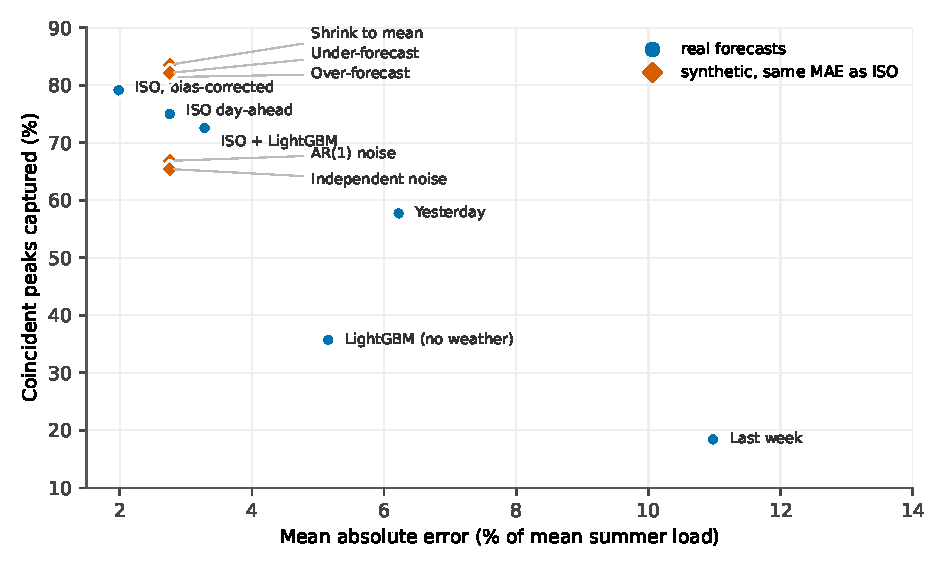
\includegraphics[width=0.92\linewidth]{fig_capture_mae.pdf}
\caption{Share of coincident-peak hours caught against mean absolute error, primary rule, averaged over \res{nMarketYears} market-years (data as published). Synthetic forecasts (diamonds) have the same error as the ISO forecast in each market-year. Alert counts differ between forecasts under this rule.}
\label{fig:cap}
\end{figure}

\begin{table}[t]
\centering
\caption{Share of coincident-peak hours caught (\%) by market, primary rule (three-hour window, five alerts per CP). The last row repeats PJM with its forecast realigned (Section~\ref{sec:offset}). Alert counts differ between forecasts under this rule.}
\label{tab:market}
\small
\setlength{\tabcolsep}{4pt}
\begin{tabular}{lrrrrrrrr}
\toprule
Market & CPs & Alerts & ISO & ISO bc & LightGBM & Yesterday & Shrink & Noise \\
\midrule
ERCOT 4CP & \res{nCPErcot} & \res{budgetErcot} & \res{capIsoErcot} & \res{capIsobcErcot} & \res{capMlErcot} & \res{capPersErcot} & \res{capShrinkErcot} & \res{capNoiseErcot} \\
PJM 5CP & \res{nCPPjm} & \res{budgetPjm} & \res{capIsoPjm} & \res{capIsobcPjm} & \res{capMlPjm} & \res{capPersPjm} & \res{capShrinkPjm} & \res{capNoisePjm} \\
NYISO & \res{nCPNyiso} & \res{budgetNyiso} & \res{capIsoNyiso} & \res{capIsobcNyiso} & \res{capMlNyiso} & \res{capPersNyiso} & \res{capShrinkNyiso} & \res{capNoiseNyiso} \\
ISO-NE & \res{nCPIsone} & \res{budgetIsone} & \res{capIsoIsone} & \res{capIsobcIsone} & \res{capMlIsone} & \res{capPersIsone} & \res{capShrinkIsone} & \res{capNoiseIsone} \\
\midrule
PJM, realigned & \res{raNCPPjm} & \res{raBudgetPjm} & \res{raCapIsoPjm} & \res{raCapIsobcPjm} & \res{raCapMlPjm} & \res{raCapPersPjm} & \res{raCapShrinkPjm} & \res{raCapNoisePjm} \\
\bottomrule
\end{tabular}
\end{table}

\subsection{But not sufficient: the shape of the error}

The five synthetic forecasts have exactly the operator forecast's error in every market-year, yet they differed widely in the peaks they caught (Figure~\ref{fig:types}). With alert counts held equal by the ex post rule, errors that keep the order of days caught nearly every peak: \res{capBiasExact}\% for a constant over- or under-forecast and \res{capShrinkExact}\% for shrink to mean. Random errors of the same size caught \res{capNoiseExact}\% (independent) and \res{capAroneExact}\% (autocorrelated). The operator's forecast, with its own error of the same size, caught \res{capIsoExact}\% (realigned \res{raCapIsoExact}\%), \res{isoPosExact}\% of the way from the random to the order-keeping end (realigned \res{raIsoPosExact}\%). At a given accuracy, then, a forecast can lose anything from none to a fifth of the peaks, and the operators' forecasts leave room for improvement that a lower error alone would not reveal. Under the rule without a running maximum, which is out of sample, the same ordering held (order-keeping \res{capShrinkNomax}--\res{capBiasNomax}\%, random \res{capAroneNomax}--\res{capNoiseNomax}\%).

H2, that compressed peaks would do worst, was not supported (one-sided $p=\res{hTwoPBias}$, \res{hTwoPUnder} and \res{hTwoPNoise}). Compression is harmless when the alert threshold is set on the forecast's own past values, because the whole forecast is compressed alike. It is harmful when the threshold comes from actual past peaks: then shrink to mean caught only \res{capShrinkActual}\% of CPs, against \res{capBiasActual}\% for a constant over-forecast, because its compressed peaks rarely reached the threshold. For the operator forecasts the two ways of setting thresholds gave similar results (ISO \res{capIso}\% and \res{capIsoActual}\%), but any forecast whose peaks are damped needs thresholds calibrated on its own scale.

\begin{figure}[t]
\centering
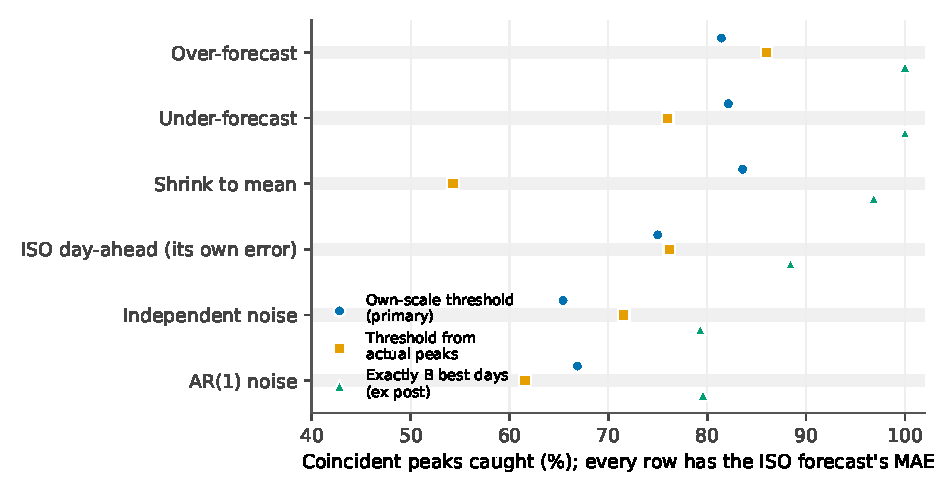
\includegraphics[width=0.95\linewidth]{fig_error_types.pdf}
\caption{Coincident peaks caught by five synthetic forecasts with exactly the ISO forecast's mean absolute error, and by the ISO forecast itself, under three ways of using a forecast: thresholds on the forecast's own scale (primary rule; alert counts differ), thresholds from actual past peaks, and the ex post choice of the budgeted number of days with the highest forecast peaks (equal alert counts). Data as published.}
\label{fig:types}
\end{figure}

\subsection{No summary score replaces a backtest}

If error is an incomplete guide, perhaps a score of how well a forecast ranks the season's top days is a better one. H3 was not supported: the top-five ranking score was associated with capture about as strongly as error was (mean $\tau=\res{hThreeTail}$ against \res{hOneTau}; one-sided $p=\res{hThreeP}$, realigned \res{raHThreeP}). Measured on the previous season, so that it could be known in advance, the two were equally informative ($\tau=\res{oosTail}$ and \res{oosMae}; exploratory).

\subsection{Operator forecasts are a strong free baseline}

H4 was supported. The ISO forecast caught at least as many CPs as LightGBM in every market and more in three: ERCOT \res{hFourIsoErcot} against \res{hFourMlErcot} of \res{hFourNErcot} CP hours, NYISO \res{hFourIsoNyiso} against \res{hFourMlNyiso} of \res{hFourNNyiso}, ISO-NE \res{hFourIsoIsone} against \res{hFourMlIsone} of \res{hFourNIsone}. In PJM the two tied at \res{hFourIsoPjm} of \res{hFourNPjm} on the data as published; realigned, the ISO forecast caught \res{raHFourIsoPjm} and was ahead in all four markets. LightGBM had no weather input, so this is a comparison with a deliberately simple model; it shows that the operators' forecasts, which are free and use weather, set the bar a paid service should clear on capture. A 28-day bias correction raised the share caught from \res{capIso}\% to \res{capIsobc}\% on the data as published, but almost all of that gain came from PJM's misaligned data: realigned, the raw and corrected operator forecasts caught \res{raCapIso}\% and \res{raCapIsobc}\%.

\subsection{A one-hour offset in PJM's public forecast}
\label{sec:offset}

An erratum to a public scorecard of EIA-930 forecasts reported that PJM's forecast is stamped one hour earlier than its demand from February 2019 \citep{guerrafilho2026scorecard}, and a separate screening by the author found the same \citep{nguyen2026eia930}. I tested it here in three ways. First, comparing each year's forecast error with the forecast shifted by up to two hours, no shift improved the forecast in ERCOT, NYISO or ISO-NE in any of \res{lagOtherN} market-years, while in PJM pairing each hour's demand with the forecast stamped one hour earlier was best in every year from 2019 (\res{lagPjmYearsBest} of \res{lagPjmYearsPost}; Figure~\ref{fig:offset}a). Realigned, PJM's annual forecast error fell from \res{lagPjmPostZero}\% to \res{lagPjmPostShift}\% of mean load, its 2016--2018 level (\res{lagPjmPre}\%). Second, the offset appeared in winter months on standard time and in summer months on daylight time alike (\res{seasonBest} of \res{seasonN} season-years since 2019), so it is not a daylight-saving error. Third, PJM's official 5CP hours for 2022--2026 \citep{pjm5cp} settle which series is shifted: EIA-930 demand peaked in the official hour on \res{offDemAt} of the \res{offN} CP days, but the forecast peaked there on only \res{offFcAt} as published and on \res{offFcRaAt} after realignment (mean distance from the official hour \res{offFcLag} and \res{offFcRaLag} hours). The demand is correctly stamped; the forecast is early.

For coincident peaks the offset matters more than the error figures suggest, because it moves the forecast peak hour. Under the primary rule the ISO forecast caught \res{pjmPubIsoPrimW3} of \res{pjmNcp} PJM CP hours as published and \res{pjmRaIsoPrimW3} realigned (Table~\ref{tab:market}). With alert counts held closer to the budget (rule without running maximum; \res{alertsNomaxPjmMin}--\res{alertsNomaxPjmMax} alerts a season against \res{budgetPjm}), it caught \res{pjmPubIsoNomaxW3} and \res{pjmRaIsoNomaxW3}, and with a one-hour curtailment window \res{pjmPubIsoNomaxW1} and \res{pjmRaIsoNomaxW1} (Figure~\ref{fig:offset}b). Both versions alerted every PJM CP day under this rule; the loss is in the hour. The bias-corrected forecast was largely immune (\res{pjmPubIsobcNomaxW3} and \res{pjmRaIsobcNomaxW3}), because a one-hour shift shows up as a stable error at each hour of the day, which the correction removes.

A backtest of PJM peak alerts on the public data would therefore understate the operator's free forecast, and a competing forecast could look better than it is. The general results above did not depend on the offset: realignment changed none of the four hypothesis outcomes.

\begin{figure}[t]
\centering
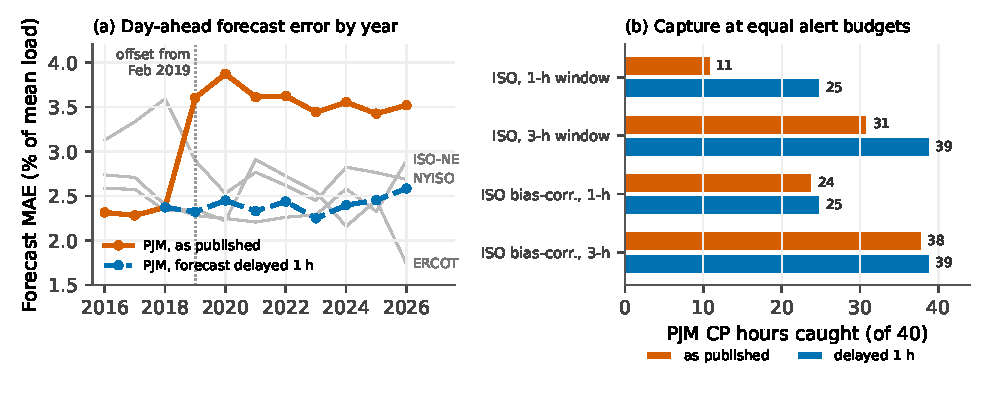
\includegraphics[width=\linewidth]{fig_pjm_offset.pdf}
\caption{PJM's day-ahead forecast in EIA-930. (a) Annual mean absolute error of each market's forecast as published (grey: ERCOT, NYISO, ISO-NE; orange: PJM) and of PJM's forecast delayed by one hour (blue). (b) PJM coincident-peak hours caught by the ISO forecast and its bias-corrected version, \res{firstYear}--\res{lastYear}, with alert counts held closer to the budget (rule without running maximum), as published and realigned.}
\label{fig:offset}
\end{figure}

\section{Implications for customers, operators and regulators}

\paragraph{Customers and vendors} Accuracy is necessary but not sufficient. Two forecasts with the same error can differ by a fifth of the peaks caught, so a vendor's claim of lower error is weak evidence that its alerts will catch more peaks, and a claim of more peaks caught is weak evidence unless the number of alerts is stated. Each CP missed is costly: in the PJM illustration above, about \$\res{illusCost} a year for a \res{illusMw}-MW load. A customer choosing a CP alert service can ask four questions:
\begin{enumerate}
\item How many peaks did the service catch in past seasons, in this market, and with how many alerts?
\item Were those results out of sample, with thresholds fixed before each season?
\item Are alert thresholds set on the forecast's own scale or on actual past peaks?
\item Was the backtest run on forecast and demand data whose alignment was checked?
\end{enumerate}

\paragraph{The operators' forecasts as a baseline} The operators' day-ahead forecasts are free, use weather, and caught at least as many peaks as a weather-free model in every market. Any paid service should be benchmarked against them on capture. A simple hour-by-hour bias correction, which any customer can compute, added little on aligned data but protected against PJM's timing error, which makes it a cheap safeguard.

\paragraph{EIA and users of EIA-930} EIA-930 is the standard public source for comparing US load forecasts across regions, and forecast evaluations on it pair the forecast and demand columns hour by hour. For PJM, the two have not been aligned since February 2019. EIA could document each balancing authority's time convention for the forecast column, check the alignment of forecast and demand routinely, and flag or correct offsets. Until then, users should check alignment themselves before any forecast evaluation: comparing the error at shifts of one hour either way, as in Figure~\ref{fig:offset}a, takes a few lines of code.

\paragraph{Regulators and tariff design} Coincident-peak charges reward customers for predicting the ranking of days and the hour of the peak, which accuracy-based comparisons do not measure. Regulators who review demand-response programmes or CP-based tariffs would be better served by evaluations in terms of peaks caught per alert. Because the CP itself can move when many customers curtail at once \citep{zhang2026cp}, the value of such forecasts may change as more load responds.

\section{Limitations}

CP hours were identified from hourly EIA-930 demand; for PJM they matched the official 5CP days in \res{offCpDays} of \res{offN} cases in 2022--2026, but ERCOT defines its peaks on 15-minute intervals and NYISO's capability period is longer than the window used here. The alert rules are stylised: real customers use intraday updates, weather forecasts and judgement. Alert counts differ between forecasts under the primary rule; the secondary rules address this, one of them ex post. The order-keeping synthetic forecasts are built from actual load and mark an upper bound rather than an achievable forecast. The machine-learning model had no weather input, and the non-operator forecasts use slightly later information than the operator forecast. In NYISO and ISO-NE, with one CP a year, each market contributes nine peaks. The dollar figure is an illustration: peak-load contributions are scaled by zone, and the charge depends on each customer's load-serving arrangement. The plan was amended five times, three times after results had been seen; all amendments and earlier results are kept with the code, and the plan and amendment timestamps are local git commits, so this is not a registered report.

\section{Conclusions}

A more accurate day-ahead load forecast catches more coincident peaks, but accuracy is not sufficient. At the operators' level of error, the shape of the error decides whether a forecast loses almost none or a fifth of the peaks, and forecasts that compress peaks need thresholds set on their own scale. The operators' free forecasts are a strong baseline. In the public EIA-930 data, PJM's forecast has been stamped one hour early relative to its demand since February 2019, which makes it look worse at finding the peak hour than it is. Peak forecasts should be judged by backtested capture at a stated number of alerts, on data whose alignment has been checked.

\section*{Data availability}
EIA-930 data are public \citep{eia930}, and PJM's 5CP reports are published annually \citep{pjm5cp}. The analysis plan with its commit history and amendment log, the code, the download script with file hashes, the official 5CP files with their hashes, and the results of every run are available at \url{\repoURL}.

\section*{CRediT authorship contribution statement}
\textbf{Thanh Van Nguyen:} Conceptualization, Methodology, Software, Formal analysis, Data curation, Writing -- original draft, Writing -- review \& editing.

\section*{Declaration of generative AI and AI-assisted technologies in the writing process}
During the preparation of this work the author used Claude Opus 5.5 (Anthropic; used in November 2026 through Claude Code) to help write and test the analysis code, search the literature and check every reference against Crossref and arXiv, obtain a referee-style critique of the draft, and draft and edit the text; its use in the research process is also described in Section 2.4. The author chose the research question, approved the analysis plan and each amendment, and checked the results. After using this tool, the author reviewed and edited the content as needed and takes full responsibility for the content of the published article.

\section*{Declaration of competing interest}
The author declares no known competing financial interests or personal relationships that could have appeared to influence the work reported in this paper.

\section*{Funding}
This research did not receive any specific grant from funding agencies in the public, commercial, or not-for-profit sectors.

\appendix

\section{Tests, budgets and robustness}
\label{app:robust}

H1 and H3 use Kendall's $\tau_b$ \citep{kendall1945ties} within each market-year, averaged over market-years, with bootstrap intervals over market-years \citep{efron1993bootstrap}; H3 compares the two averages with a paired bootstrap. H2 uses one-sided Wilcoxon signed-rank tests \citep{wilcoxon1945individual} with Holm's correction \citep{holm1979simple}. Budgets of three and eight alerts per CP and curtailment windows of one and five hours are robustness checks.

Table~\ref{tab:robust} reports the correlations and the capture of the synthetic forecasts under the secondary rules, budgets and windows (data as published). Across all \res{nConfigs} combinations of rule, budget and window, the mean correlation between error and capture ranged from \res{tauAllMin} to \res{tauAllMax} (realigned \res{raTauAllMin} to \res{raTauAllMax}), and that between the ranking score and capture from \res{tailAllMin} to \res{tailAllMax}. Excluding 2020 changed neither ($\tau=\res{tauNoCovid}$ and \res{tailNoCovid}).

\begin{table}[h]
\centering
\caption{Mean within-market-year Kendall $\tau$ of capture with error and with the top-five ranking score, and capture (\%) of the same-error synthetic forecasts, under the primary and secondary configurations (alerts per CP; window in hours). Data as published.}
\label{tab:robust}
\small
\setlength{\tabcolsep}{4pt}
\begin{tabular}{lrrrrrrr}
\toprule
Configuration & $\tau$ error & $\tau$ rank & Over & Under & Shrink & Noise & AR(1) \\
\midrule
Primary (own scale, $\times5$, 3 h) & \res{hOneTau} & \res{hThreeTail} & \res{capBias} & \res{capUnder} & \res{capShrink} & \res{capNoise} & \res{capArone} \\
No running maximum & \res{tauNomax} & \res{tailNomax} & \res{capBiasNomax} & \res{capUnderNomax} & \res{capShrinkNomax} & \res{capNoiseNomax} & \res{capAroneNomax} \\
Threshold from actual peaks & \res{tauActual} & \res{tailActual} & \res{capBiasActual} & \res{capUnderActual} & \res{capShrinkActual} & \res{capNoiseActual} & \res{capAroneActual} \\
Exactly budgeted days (ex post) & \res{tauExact} & \res{tailExact} & \res{capBiasExact} & \res{capUnderExact} & \res{capShrinkExact} & \res{capNoiseExact} & \res{capAroneExact} \\
Budget $\times3$ & \res{tauMthree} & \res{tailMthree} & \res{capBiasMthree} & \res{capUnderMthree} & \res{capShrinkMthree} & \res{capNoiseMthree} & \res{capAroneMthree} \\
Budget $\times8$ & \res{tauMeight} & \res{tailMeight} & \res{capBiasMeight} & \res{capUnderMeight} & \res{capShrinkMeight} & \res{capNoiseMeight} & \res{capAroneMeight} \\
Window 1 h & \res{tauWone} & \res{tailWone} & \res{capBiasWone} & \res{capUnderWone} & \res{capShrinkWone} & \res{capNoiseWone} & \res{capAroneWone} \\
Window 5 h & \res{tauWfive} & \res{tailWfive} & \res{capBiasWfive} & \res{capUnderWfive} & \res{capShrinkWfive} & \res{capNoiseWfive} & \res{capAroneWfive} \\
\bottomrule
\end{tabular}
\end{table}

\section{Amendments to the analysis plan}
\label{app:amend}

The plan was committed after one data file had been downloaded to check access. Amendment~1 fixed a coding error found in a pipeline check on ERCOT 2018--2019. Amendment~2, after that check and before the full run, normalised thresholds by trailing mean load, because load growth made the calibrated rules issue far more alerts than budgeted, and added the exactly-budgeted rule; the check's capture results had been seen. Amendment~3, after the full run, screened recording errors, prompted by a 2.1-billion-MW value in PJM's 2021 data. Amendment~4, after an internal referee-style review, loosened that screen (its first version also removed genuine heat-wave peaks), implemented the pre-specified exclusion of market-years with incomplete CP days, corrected the holiday calendar, made the synthetic forecasts' error exactly equal to the ISO forecast's, and added the exploratory analyses marked as such; it changed H3 from supported to not supported (H1 $\tau$ before any screening: \res{vOneTau}). Amendment~5, logged before its results were seen, reran the whole analysis with PJM's forecast delayed by one hour from February 2019 and added the alignment check; after a further internal review it added the comparison with PJM's official 5CP hours and the seasonal check (Section~\ref{sec:offset}). The results on the data as published were kept and are reported throughout.

\begin{thebibliography}{25}
\expandafter\ifx\csname natexlab\endcsname\relax\def\natexlab#1{#1}\fi
\providecommand{\url}[1]{\texttt{#1}}
\providecommand{\href}[2]{#2}
\providecommand{\path}[1]{#1}
\providecommand{\DOIprefix}{doi:}
\providecommand{\ArXivprefix}{arXiv:}
\providecommand{\URLprefix}{URL: }
\providecommand{\Pubmedprefix}{pmid:}
\providecommand{\doi}[1]{\href{http://dx.doi.org/#1}{\path{#1}}}
\providecommand{\Pubmed}[1]{\href{pmid:#1}{\path{#1}}}
\providecommand{\bibinfo}[2]{#2}
\ifx\xfnm\relax \def\xfnm[#1]{\unskip,\space#1}\fi
%Type = Article
\bibitem[{Carmona et~al.(2026)Carmona, Yang and Zeng}]{carmona2026cp}
\bibinfo{author}{Carmona, R.}, \bibinfo{author}{Yang, X.}, \bibinfo{author}{Zeng, C.}, \bibinfo{year}{2026}.
\newblock \bibinfo{title}{Coincident peak prediction for capacity and transmission charge reduction}.
\newblock \bibinfo{journal}{Energy Systems} \DOIprefix\doi{10.1007/s12667-026-00788-1}.
%Type = Book
\bibitem[{Efron and Tibshirani(1994)}]{efron1993bootstrap}
\bibinfo{author}{Efron, B.}, \bibinfo{author}{Tibshirani, R.}, \bibinfo{year}{1994}.
\newblock \bibinfo{title}{An Introduction to the Bootstrap}.
\newblock \bibinfo{publisher}{Chapman and Hall/CRC}.
\newblock \DOIprefix\doi{10.1201/9780429246593}.
%Type = Article
\bibitem[{Gneiting(2011)}]{gneiting2011point}
\bibinfo{author}{Gneiting, T.}, \bibinfo{year}{2011}.
\newblock \bibinfo{title}{Making and evaluating point forecasts}.
\newblock \bibinfo{journal}{Journal of the American Statistical Association} \bibinfo{volume}{106}, \bibinfo{pages}{746–762}.
\newblock \DOIprefix\doi{10.1198/jasa.2011.r10138}.
%Type = Misc
\bibitem[{Guerra~Filho(2026)}]{guerrafilho2026scorecard}
\bibinfo{author}{Guerra~Filho, R.W.C.}, \bibinfo{year}{2026}.
\newblock \bibinfo{title}{Day-ahead load forecast accuracy of {U.S.} balancing authorities, 2015--2026: a scorecard from public {EIA-930} data}.
\newblock \bibinfo{howpublished}{Cardinal Grid Notes, No. 1, version 1.3 (erratum of 21 September 2026), Zenodo}.
\newblock \DOIprefix\doi{10.5281/zenodo.22883589}.
%Type = Article
\bibitem[{Hobbs et~al.(1999)Hobbs, Jitprapaikulsarn, Konda, Chankong, Loparo and Maratukulam}]{hobbs1999value}
\bibinfo{author}{Hobbs, B.}, \bibinfo{author}{Jitprapaikulsarn, S.}, \bibinfo{author}{Konda, S.}, \bibinfo{author}{Chankong, V.}, \bibinfo{author}{Loparo, K.}, \bibinfo{author}{Maratukulam, D.}, \bibinfo{year}{1999}.
\newblock \bibinfo{title}{Analysis of the value for unit commitment of improved load forecasts}.
\newblock \bibinfo{journal}{IEEE Transactions on Power Systems} \bibinfo{volume}{14}, \bibinfo{pages}{1342–1348}.
\newblock \DOIprefix\doi{10.1109/59.801894}.
%Type = Article
\bibitem[{Holm(1979)}]{holm1979simple}
\bibinfo{author}{Holm, S.}, \bibinfo{year}{1979}.
\newblock \bibinfo{title}{A simple sequentially rejective multiple test procedure}.
\newblock \bibinfo{journal}{Scandinavian Journal of Statistics} \bibinfo{volume}{6}, \bibinfo{pages}{65--70}.
%Type = Article
\bibitem[{Hong and Fan(2016)}]{hong2016probabilistic}
\bibinfo{author}{Hong, T.}, \bibinfo{author}{Fan, S.}, \bibinfo{year}{2016}.
\newblock \bibinfo{title}{Probabilistic electric load forecasting: A tutorial review}.
\newblock \bibinfo{journal}{International Journal of Forecasting} \bibinfo{volume}{32}, \bibinfo{pages}{914–938}.
\newblock \DOIprefix\doi{10.1016/j.ijforecast.2015.11.011}.
%Type = Article
\bibitem[{Hyndman and Koehler(2006)}]{hyndman2006another}
\bibinfo{author}{Hyndman, R.J.}, \bibinfo{author}{Koehler, A.B.}, \bibinfo{year}{2006}.
\newblock \bibinfo{title}{Another look at measures of forecast accuracy}.
\newblock \bibinfo{journal}{International Journal of Forecasting} \bibinfo{volume}{22}, \bibinfo{pages}{679–688}.
\newblock \DOIprefix\doi{10.1016/j.ijforecast.2006.03.001}.
%Type = Inproceedings
\bibitem[{Ke et~al.(2017)Ke, Meng, Finley, Wang, Chen, Ma, Ye and Liu}]{ke2017lightgbm}
\bibinfo{author}{Ke, G.}, \bibinfo{author}{Meng, Q.}, \bibinfo{author}{Finley, T.}, \bibinfo{author}{Wang, T.}, \bibinfo{author}{Chen, W.}, \bibinfo{author}{Ma, W.}, \bibinfo{author}{Ye, Q.}, \bibinfo{author}{Liu, T.Y.}, \bibinfo{year}{2017}.
\newblock \bibinfo{title}{{LightGBM}: A highly efficient gradient boosting decision tree}, in: \bibinfo{booktitle}{Advances in Neural Information Processing Systems 30}, pp. \bibinfo{pages}{3146--3154}.
%Type = Article
\bibitem[{KENDALL(1945)}]{kendall1945ties}
\bibinfo{author}{KENDALL, M.G.}, \bibinfo{year}{1945}.
\newblock \bibinfo{title}{The treatment of ties in ranking problems}.
\newblock \bibinfo{journal}{Biometrika} \bibinfo{volume}{33}, \bibinfo{pages}{239–251}.
\newblock \DOIprefix\doi{10.1093/biomet/33.3.239}.
%Type = Article
\bibitem[{Liu et~al.(2013)Liu, Wierman, Chen, Razon and Chen}]{liu2013datacenter}
\bibinfo{author}{Liu, Z.}, \bibinfo{author}{Wierman, A.}, \bibinfo{author}{Chen, Y.}, \bibinfo{author}{Razon, B.}, \bibinfo{author}{Chen, N.}, \bibinfo{year}{2013}.
\newblock \bibinfo{title}{Data center demand response: Avoiding the coincident peak via workload shifting and local generation}.
\newblock \bibinfo{journal}{Performance Evaluation} \bibinfo{volume}{70}, \bibinfo{pages}{770–791}.
\newblock \DOIprefix\doi{10.1016/j.peva.2013.08.014}.
%Type = Article
\bibitem[{Murphy(1993)}]{murphy1993good}
\bibinfo{author}{Murphy, A.H.}, \bibinfo{year}{1993}.
\newblock \bibinfo{title}{What is a good forecast? an essay on the nature of goodness in weather forecasting}.
\newblock \bibinfo{journal}{Weather and Forecasting} \bibinfo{volume}{8}, \bibinfo{pages}{281–293}.
\newblock \DOIprefix\doi{10.1175/1520-0434(1993)008<0281:wiagfa>2.0.co;2}.
%Type = Article
\bibitem[{Murphy and Winkler(1987)}]{murphy1987general}
\bibinfo{author}{Murphy, A.H.}, \bibinfo{author}{Winkler, R.L.}, \bibinfo{year}{1987}.
\newblock \bibinfo{title}{A general framework for forecast verification}.
\newblock \bibinfo{journal}{Monthly Weather Review} \bibinfo{volume}{115}, \bibinfo{pages}{1330–1338}.
\newblock \DOIprefix\doi{10.1175/1520-0493(1987)115<1330:agfffv>2.0.co;2}.
%Type = Misc
\bibitem[{Nguyen(2026)}]{nguyen2026eia930}
\bibinfo{author}{Nguyen, T.V.}, \bibinfo{year}{2026}.
\newblock \bibinfo{title}{Recording errors in {EIA-930} hourly demand and forecast data and their effect on forecast evaluation}.
\newblock \bibinfo{note}{Manuscript under review, IEEE ISIE 2027. Code: \url{https://github.com/Thanh-Van-2001/eia930-quality}}.
%Type = Misc
\bibitem[{{PJM Interconnection}(2025)}]{pjm2025bra}
\bibinfo{author}{{PJM Interconnection}}, \bibinfo{year}{2025}.
\newblock \bibinfo{title}{2026/2027 {RPM} base residual auction results}.
\newblock \bibinfo{note}{Report, July 2025. \url{https://www.pjm.com/-/media/DotCom/markets-ops/rpm/rpm-auction-info/2026-2027/2026-2027-bra-report.pdf}}.
%Type = Misc
\bibitem[{{PJM Interconnection}(2026a)}]{pjm_m19}
\bibinfo{author}{{PJM Interconnection}}, \bibinfo{year}{2026}a.
\newblock \bibinfo{title}{{PJM} manual 19: Load forecasting and analysis}.
%Type = Misc
\bibitem[{{PJM Interconnection}(2026b)}]{pjm5cp}
\bibinfo{author}{{PJM Interconnection}}, \bibinfo{year}{2026}b.
\newblock \bibinfo{title}{Summer peaks and {5CPs}, 2022--2026}.
\newblock \bibinfo{note}{Annual reports ``Summer YYYY Peaks and 5CPs'', PJM Resource Adequacy Planning; files and SHA-256 hashes in the study repository}.
%Type = Misc
\bibitem[{{Public Utility Commission of Texas}(2026)}]{puct25192}
\bibinfo{author}{{Public Utility Commission of Texas}}, \bibinfo{year}{2026}.
\newblock \bibinfo{title}{Substantive rule {\S}25.192: Transmission service rates}.
\newblock \bibinfo{note}{Texas Administrative Code, Title 16, Chapter 25}.
%Type = Article
\bibitem[{Ranaweera et~al.(1997)Ranaweera, Karady and Farmer}]{ranaweera1997economic}
\bibinfo{author}{Ranaweera, D.}, \bibinfo{author}{Karady, G.}, \bibinfo{author}{Farmer, R.}, \bibinfo{year}{1997}.
\newblock \bibinfo{title}{Economic impact analysis of load forecasting}.
\newblock \bibinfo{journal}{IEEE Transactions on Power Systems} \bibinfo{volume}{12}, \bibinfo{pages}{1388–1392}.
\newblock \DOIprefix\doi{10.1109/59.630486}.
%Type = Article
\bibitem[{Ruggles et~al.(2020)Ruggles, Farnham, Tong and Caldeira}]{ruggles2020eia}
\bibinfo{author}{Ruggles, T.H.}, \bibinfo{author}{Farnham, D.J.}, \bibinfo{author}{Tong, D.}, \bibinfo{author}{Caldeira, K.}, \bibinfo{year}{2020}.
\newblock \bibinfo{title}{Developing reliable hourly electricity demand data through screening and imputation}.
\newblock \bibinfo{journal}{Scientific Data} \bibinfo{volume}{7}.
\newblock \DOIprefix\doi{10.1038/s41597-020-0483-x}.
%Type = Article
\bibitem[{Skiles et~al.(2023)Skiles, Rhodes and Webber}]{skiles2023peak}
\bibinfo{author}{Skiles, M.J.}, \bibinfo{author}{Rhodes, J.D.}, \bibinfo{author}{Webber, M.E.}, \bibinfo{year}{2023}.
\newblock \bibinfo{title}{Perspectives on peak demand: How is ercot peak electric load evolving in the context of changing weather and heating electrification?}
\newblock \bibinfo{journal}{The Electricity Journal} \bibinfo{volume}{36}, \bibinfo{pages}{107254}.
\newblock \DOIprefix\doi{10.1016/j.tej.2023.107254}.
%Type = Misc
\bibitem[{{U.S. Energy Information Administration}(2026)}]{eia930}
\bibinfo{author}{{U.S. Energy Information Administration}}, \bibinfo{year}{2026}.
\newblock \bibinfo{title}{Hourly electric grid monitor ({Form EIA-930}): six-month balance files}.
\newblock \bibinfo{note}{Accessed November 2026}.
%Type = Article
\bibitem[{Wilcoxon(1945)}]{wilcoxon1945individual}
\bibinfo{author}{Wilcoxon, F.}, \bibinfo{year}{1945}.
\newblock \bibinfo{title}{Individual comparisons by ranking methods}.
\newblock \bibinfo{journal}{Biometrics Bulletin} \bibinfo{volume}{1}, \bibinfo{pages}{80}.
\newblock \DOIprefix\doi{10.2307/3001968}.
%Type = Article
\bibitem[{Zarnikau and Thal(2013)}]{zarnikau2013response}
\bibinfo{author}{Zarnikau, J.}, \bibinfo{author}{Thal, D.}, \bibinfo{year}{2013}.
\newblock \bibinfo{title}{The response of large industrial energy consumers to four coincident peak (4cp) transmission charges in the texas (ercot) market}.
\newblock \bibinfo{journal}{Utilities Policy} \bibinfo{volume}{26}, \bibinfo{pages}{1–6}.
\newblock \DOIprefix\doi{10.1016/j.jup.2013.04.004}.
%Type = Misc
\bibitem[{Zhang et~al.(2026)Zhang, Zhao, Diao, Byers, Chen, Cansever and Xie}]{zhang2026cp}
\bibinfo{author}{Zhang, Q.}, \bibinfo{author}{Zhao, S.}, \bibinfo{author}{Diao, L.}, \bibinfo{author}{Byers, C.}, \bibinfo{author}{Chen, Y.}, \bibinfo{author}{Cansever, D.}, \bibinfo{author}{Xie, L.}, \bibinfo{year}{2026}.
\newblock \bibinfo{title}{Modeling coincident peak pricing in electricity markets: challenges and peak shaving effectiveness}.
\newblock \href{http://arxiv.org/abs/2605.16794}{{\tt arXiv:2605.16794}}. \bibinfo{note}{arXiv preprint arXiv:2605.16794}.

\end{thebibliography}

\end{document}
